%Se podrá presentar en dos Capítulos separados: Capítulo 4: Resultados y Capítulo 5: Discusión

%HIPÓTESIS: la linealidad se mantiene o no con la escala
\color{black} 
\section {Bloque/Núcleo 1-A1-Propuesta de relevamiento por imágenes RGB de las reservas de la provincia de Misiones}

Con base en todos los cálculos, es posible establecer una comparación entre las distintas opciones de plataforma de sensado remoto, según el área relevada.
%% No olvidar mencionar que, por simplicidad en los cálculos se considera cada área como si fuera un cuadrado 
%%
En las tablas \ref{tab:yaboty}, \ref{tab:sanse} y \ref{tab:profundidad} se sumarizan los resultados, donde se puede observar de forma clara que para el caso de superficies relevadas de pocas hectáreas, el costo de obtención de las imágenes es significativamente inferior al de las imágenes satelitales. Esto se debe fundamentalmente a que la adquisición de imágenes satelitales requiere de una superficie mínima, 25 kilómetros cuadrados si las imágenes son de archivo (> 90 días)\cite{noauthor_satellite_2020}. Ya para el caso de superficies mayores como la reserva Yaboty, el costo total de captura de imágenes equipara e incluso supera al de imágenes satelitales. No solo termina siendo más oneroso el relevamiento fotográfico aéreo con VANT en grandes superficies, ya que adicionalmente se debe tener en cuenta la limitación de autonomía de esos vehículos, que generalmente no superan la media hora \cite{noauthor_dji_nodate}, o la hora de autonomía en algunos casos \cite{noauthor_specs_nodate}, aunque hay algunos que llegan a dos horas de autonomía \cite{noauthor_us-1_nodate}. Esto indudablemente afecta al flujo de trabajo por la necesaria reposición de baterías, a la vez que deben establecerse numerosas bases operativas en la medida en que se va avanzando con el relevamiento del terreno. Otra limitación que se suma a los VANT es el alcance que tiene el mando de control. Los VANT comerciales más difundidos suelen tener alcances de hasta 10 km \cite{noauthor_dji_nodate} por lo que esto debe ser tenido en cuenta en la extensión del área a relevar. Por otro lado en el caso de las aeronaves tripuladas puede resultar muy inconvenientes en términos de erogación de dinero cuando se trata de pequeñas extensiones cuyo sobrevuelo de relevamiento no sobrepasa la hora de duración, ya que hay que sumar a toda la operatoria el traslado de la aeronave desde y hacia el aeródromo de base. Resulta evidente que será mayor la incidencia en el costo final la parte que corresponde al traslado en sí, si la superficie a ser relevada es de pocas hectáreas. En la provincia de Misiones existen en un radio menor a cincuenta kilómetros a las tres reservas analizadas algunos aeródromos o pistas que pueden usarse como base.
%\subsubsection{Cálculo presupuestario} %revisar si corresponde que quede aquí, en relación al párrafo precedente
Partiendo de las características del terreno a relevar (su extensión) y de la plataforma usada para la captura (dron con cámara/sensor) es posible acotar un marco presupuestario para llevar a cabo la tarea. Con los datos recabados puede afirmarse que para un relevamiento aéreo de un área pequeña de veinte hectáreas, es conveniente un VANT, ya que el costo total no excedería los 10 dólares, mientras que en un avión tripulado el costo total sería por lo menos diez veces, y una imagen satelital tendría un costo de 375 dólares. En el caso de un área un poco más grande, de cien hectáreas, el costo total con VANT sigue siendo más bajo que con las otras plataformas, con menos de 50 dólares. Finalmente para el caso de un área mucho más grande, de varios miles de hectáreas como la reserva Yaboty, se torna más conveniente el avión tripulado con alrededor de 20 mil dólares estadounidenses, un poco más que la mitad de lo que cuesta la imagen satelital, y muy por debajo del costo del VANT, que supera holgadamente el millón de dólares.
% Please add the following required packages to your document preamble:
% \usepackage{multirow}
% \usepackage[table,xcdraw]{xcolor}
% Beamer presentation requires \usepackage{colortbl} instead of \usepackage[table,xcdraw]{xcolor}
% \usepackage[normalem]{ulem}
% \useunder{\uline}{\ul}{}
\begin{table}[]
\centering
\caption{Tabla comparativa de tiempos y costos de relevamiento para la reserva Yaboty}
\label{tab:yaboty}
\begin{tabular}{cclll}
\hline
\multicolumn{2}{c}{} &
  \multicolumn{3}{c}{\cellcolor[HTML]{F4B084}\textbf{Yaboty}} \\ \hline
\multicolumn{1}{l}{} &
  {\ul } &
  \cellcolor[HTML]{F4B084}tiempo {[}h{]} &
  \cellcolor[HTML]{F4B084}\$ &
  \cellcolor[HTML]{F4B084}\% \\
\cellcolor[HTML]{9BC2E6} &
  \cellcolor[HTML]{9BC2E6}{\color[HTML]{0563C1} Pleiades} &
   &
  37.500,00 USD &
   \\
\cellcolor[HTML]{9BC2E6} &
  \cellcolor[HTML]{9BC2E6}{\color[HTML]{0563C1} Satellogic} &
   &
  37.500,00 USD &
   \\
\multirow{-3}{*}{\cellcolor[HTML]{9BC2E6}Satélite} & \cellcolor[HTML]{9BC2E6}{\color[HTML]{0563C1} IKONOS} &        & 37.500,00 USD & \multirow{-3}{*}{}  \\
\cellcolor[HTML]{70AD47} &
  \cellcolor[HTML]{70AD47}{\color[HTML]{0563C1} avion} &
  69,13 &
  16.590,65 USD &
  \textgreater{}90,00 \\
\multirow{-2}{*}{\cellcolor[HTML]{70AD47}Aeronave} &
  \cellcolor[HTML]{70AD47} {\color[HTML]{0563C1}helicoptero} &
   &
   &
  \textgreater{}90,00 \\
\cellcolor[HTML]{FFC000} &
  \cellcolor[HTML]{FFC000}{\color[HTML]{0563C1} mavic   3m} &
  144,09 &
  28.098,33 USD &
  \textgreater{}90,00 \\
\cellcolor[HTML]{FFC000} &
  \cellcolor[HTML]{FFC000}{\color[HTML]{0563C1} asesor/9} &
  361,11 &
  70.416,36 USD &
  \textgreater{}90,00 \\
\multirow{-3}{*}{\cellcolor[HTML]{FFC000}VANT}     & \cellcolor[HTML]{FFC000}{\color[HTML]{0563C1} mini 2} & 314,23 & 61.275,69 USD & \textgreater{}90,01 \\ 
\end{tabular}
\end{table}

\begin{table}[]
\centering
\caption{Tabla comparativa de tiempos y costos de relevamiento para la reserva San Sebastián}
\label{tab:sanse}
\begin{tabular}{ccccc}
\hline
\multicolumn{2}{c}{} &
  \multicolumn{3}{c}{\cellcolor[HTML]{F4B084}\textbf{San   Sebastián}} \\ \hline
\multicolumn{1}{l}{} &
  {\ul } &
  \cellcolor[HTML]{F4B084}tiempo {[}min{]} &
  \cellcolor[HTML]{F4B084}\$ &
  \cellcolor[HTML]{F4B084}\% \\
\cellcolor[HTML]{9BC2E6} &
  \cellcolor[HTML]{9BC2E6}{\color[HTML]{0563C1} Pleiades} &
   &
  375,00 USD &
   \\
\cellcolor[HTML]{9BC2E6} &
  \cellcolor[HTML]{9BC2E6}{\color[HTML]{0563C1} Satellogic} &
   &
  375,00 USD &
   \\
\multirow{-3}{*}{\cellcolor[HTML]{9BC2E6}Satélite} &
  \cellcolor[HTML]{9BC2E6}{\color[HTML]{0563C1} IKONOS} &
   &
  375,00 USD &
  \multirow{-3}{*}{} \\
\cellcolor[HTML]{70AD47} &
  \cellcolor[HTML]{70AD47}{\color[HTML]{0563C1} avion} &
  2,24 &
  8,97 USD &
  \textgreater{}90,00 \\
\multirow{-2}{*}{\cellcolor[HTML]{70AD47}Aeronave} &
  \cellcolor[HTML]{70AD47}{\color[HTML]{0563C1}helicoptero }&
   &
   &
  \textgreater{}90,00 \\
\cellcolor[HTML]{FFC000} &
  \cellcolor[HTML]{FFC000}{\color[HTML]{0563C1} mavic   3m} &
  5,12 &
  16,63 USD &
  \textgreater{}90,00 \\
\cellcolor[HTML]{FFC000} &
  \cellcolor[HTML]{FFC000}{\color[HTML]{0563C1} asesor/9} &
  10,38 &
  33,73 USD &
  \textgreater{}90,00 \\
\multirow{-3}{*}{\cellcolor[HTML]{FFC000}VANT} &
  \cellcolor[HTML]{FFC000}{\color[HTML]{0563C1} mini 2} &
  9,34 &
  30,37 USD &
  \textgreater{}90,01 \\ %\cline{2-5} 
\end{tabular}
\end{table}

\begin{table}[]
\centering
\caption{Tabla comparativa de tiempos y costos de relevamiento para la reserva Profundidad}
\label{tab:profundidad}
\begin{tabular}{cclll}
\hline
\multicolumn{2}{c}{} &
  \multicolumn{3}{c}{l}{\cellcolor[HTML]{F4B084}\textbf{Profundidad}} \\ \hline
\multicolumn{1}{l}{} &
  {\ul } &
  \cellcolor[HTML]{F4B084}tiempo {[}min{]} &
  \cellcolor[HTML]{F4B084}\$ &
  \cellcolor[HTML]{F4B084}\% \\
\cellcolor[HTML]{9BC2E6} &
  \cellcolor[HTML]{9BC2E6}{\color[HTML]{0563C1} Pleiades} &
   &
  375,00 USD &
   \\
\cellcolor[HTML]{9BC2E6} &
  \cellcolor[HTML]{9BC2E6}{\color[HTML]{0563C1} Satellogic} &
   &
  375,00 USD &
   \\
\multirow{-3}{*}{\cellcolor[HTML]{9BC2E6}Satélite} &
  \cellcolor[HTML]{9BC2E6}{\color[HTML]{0563C1} IKONOS} &
   &
  375,00 USD &
  \multirow{-3}{*}{} \\
\cellcolor[HTML]{70AD47} &
  \cellcolor[HTML]{70AD47}{\color[HTML]{0563C1} avion} &
  0,42 &
  1,67 USD &
  \textgreater{}90,00 \\
\multirow{-2}{*}{\cellcolor[HTML]{70AD47}Aeronave} &
  \cellcolor[HTML]{70AD47} {\color[HTML]{0563C1}helicoptero} &
   &
   &
  \textgreater{}90,00 \\
\cellcolor[HTML]{FFC000} &
  \cellcolor[HTML]{FFC000}{\color[HTML]{0563C1} mavic   3m} &
  1,22 &
  3,98 USD &
  \textgreater{}90,00 \\
\cellcolor[HTML]{FFC000} &
  \cellcolor[HTML]{FFC000}{\color[HTML]{0563C1} asesor/9} &
  2,19 &
  7,13 USD &
  \textgreater{}90,00 \\
\multirow{-3}{*}{\cellcolor[HTML]{FFC000}VANT} &
  \cellcolor[HTML]{FFC000}{\color[HTML]{0563C1} mini 2} &
  2,25 &
  7,31 USD &
  \textgreater{}90,01 \\ 
\end{tabular}
\end{table}

%agregar gráfico final
\begin{figure}[h!]
    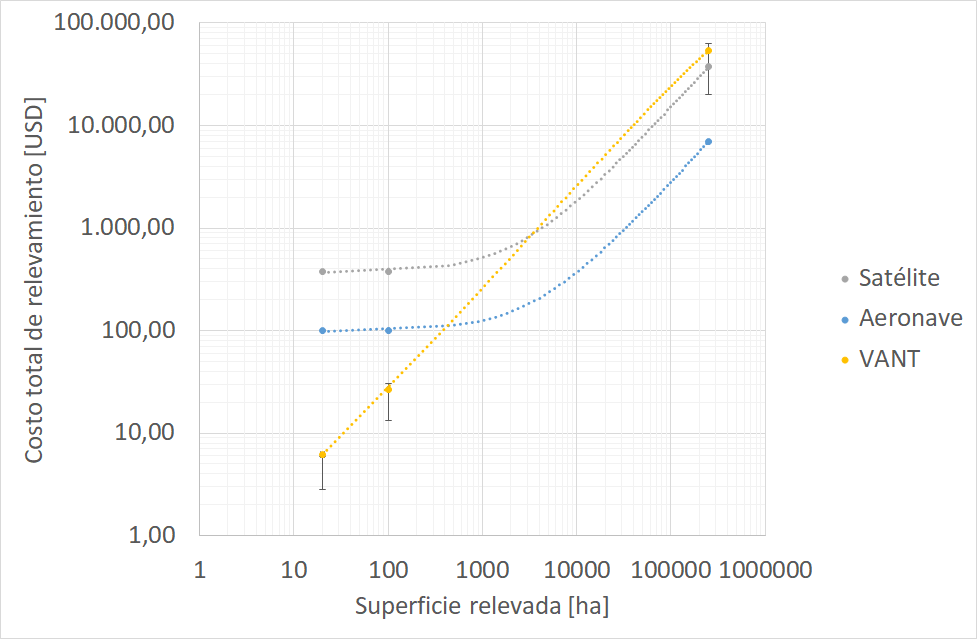
\includegraphics[width=\textwidth]{Imagenes/grafico bloque 1.png}
     \hfill
     \caption{Gráfico comparativo de costo de relevamiento con distintas plataformas versus superficie relevada}
    \label{grafico_comparativo}
\end{figure}

En la figura \ref{grafico_comparativo} se muestra un gráfico en el que se expone cómo varía el costo de relevamiento expresado en dólares estadounidenses en relación a la superficie relevada, expresada en hectáreas, según la plataforma usada, VANT, aeronaves tripuladas o satélites. Como se observa, en el caso de los VANT es claramente inferior el costo cuando se trata de superficies menores a mil hectáreas. A partir de ese valor el costo de relevamiento se asemeja al de la obtención de imágenes satelitales. Con este gráfico resulta evidente la conveniencia del uso de VANT para relevar las pequeñas reservas públicas y privadas en la provincia de Misiones.

\section{ Propuesta de Herramientas de Bajo Costo (Económico y Computacional) para el relevamiento del bosque atlántico}
%\subsection{RESULTADOS Relación de iluminación natural con histogramas de color}
%Con el objeto de evaluar la correspondiente afectación en el histograma de las imágenes capturadas respecto a las condiciones de iluminación natural, se hicieron varias capturas en distintos horarios durante varios días desde una posición fija a un determinado objeto (un árbol de palta) y se midió la iluminancia usando un luxómetro.
\color{cyan} %color de texto con 70-80 % o más de avance
\subsection{RESULTADOS Replicación del paper de Wagner}
Con base en el trabajo realizado por \cite{hubert_wagner_individual_2018}, se llevó a cabo un análisis de desempeño del algoritmo de procesamiento morfológico de imágenes mediante la técnica de "Gridsearch", evaluando diferentes valores de parámetros. En la figura \ref{Rollingball} se muestran los resultados del análisis para diferentes tamaños de ventana en  píxeles. En la figura \ref{segundaoscuros} se visualizan los resultados para distintos valores de percentil en la etapa de segunda selección de objetos oscuros. En la figura \ref{pequenoshuecos} se observan los resultados del procesamiento para hallar pequeños huecos en grandes copas, usando distintos valores de percentil. 

\begin{figure}[h!]
    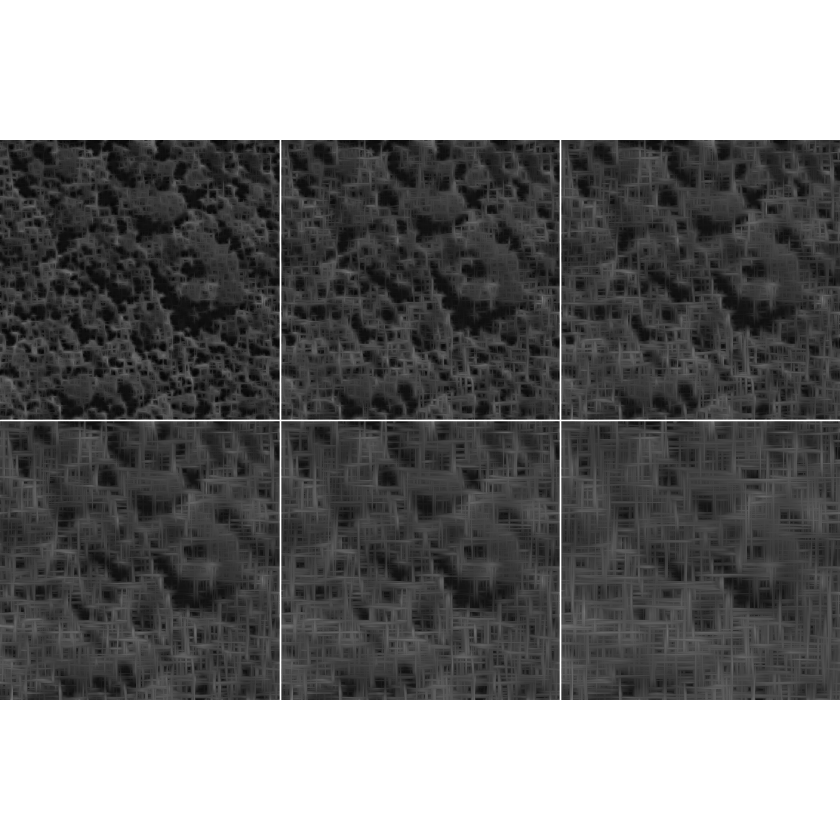
\includegraphics[width=\textwidth]{Imagenes/Resultados script morfologico/GS04.png}
     \hfill
     \caption{Resultado de Rollingball para tamaños de ventana de 6,9,12,15,18 y 24 píxeles}
    \label{Rollingball}
\end{figure}

\begin{figure}[h!]
    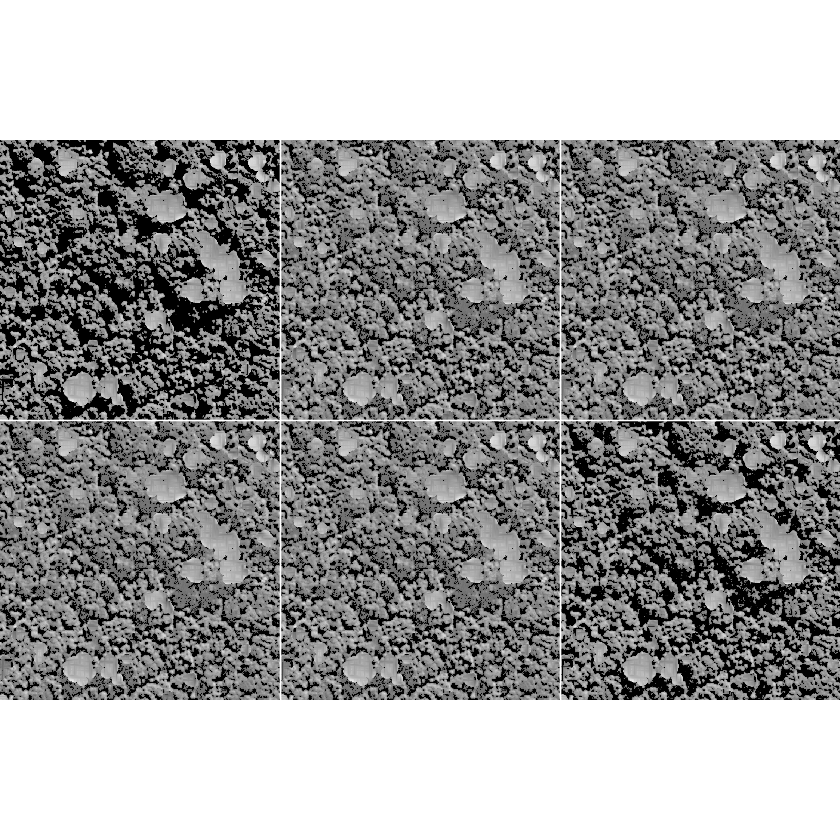
\includegraphics[width=\textwidth]{Imagenes/Resultados script morfologico/GS06.png}
     \hfill
     \caption{Resultado de la segunda selección de objetos oscuros con distintos valores de percentil, 99, 0,1, 1, 10, 50 y 90 }
    \label{segundaoscuros}
\end{figure}

\begin{figure}[h!]
    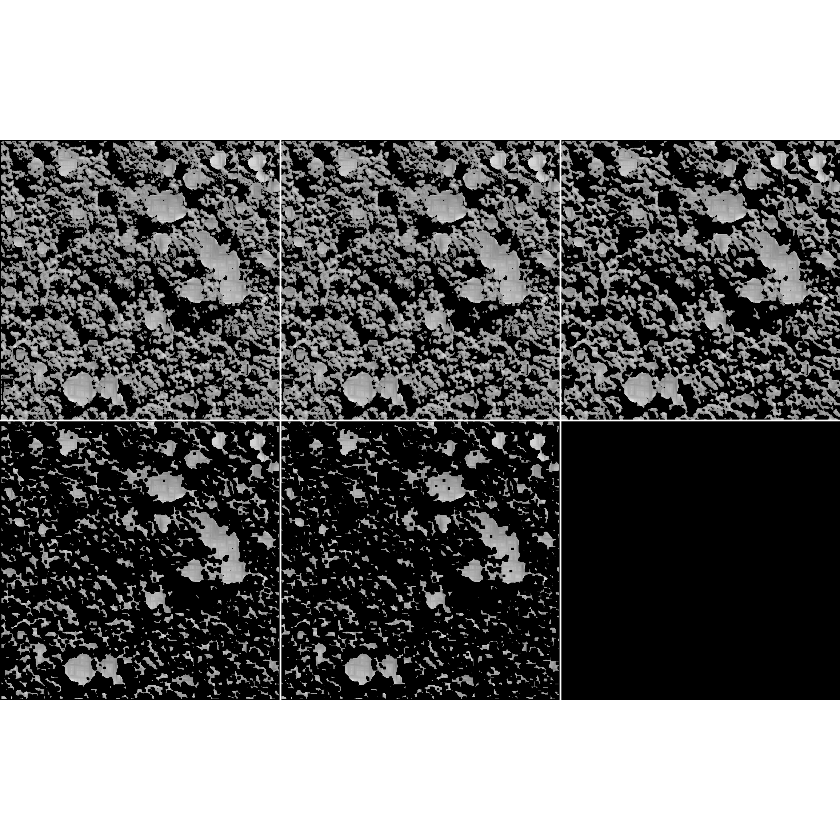
\includegraphics[width=\textwidth]{Imagenes/Resultados script morfologico/GS07.png}
     \hfill
     \caption{Resultado de la búsqueda de pequeños huecos con distintos valores de percentil, 10, 30, 50, 75, 80 y 90 }
    \label{pequenoshuecos}
\end{figure}

\begin{figure}[h!]
    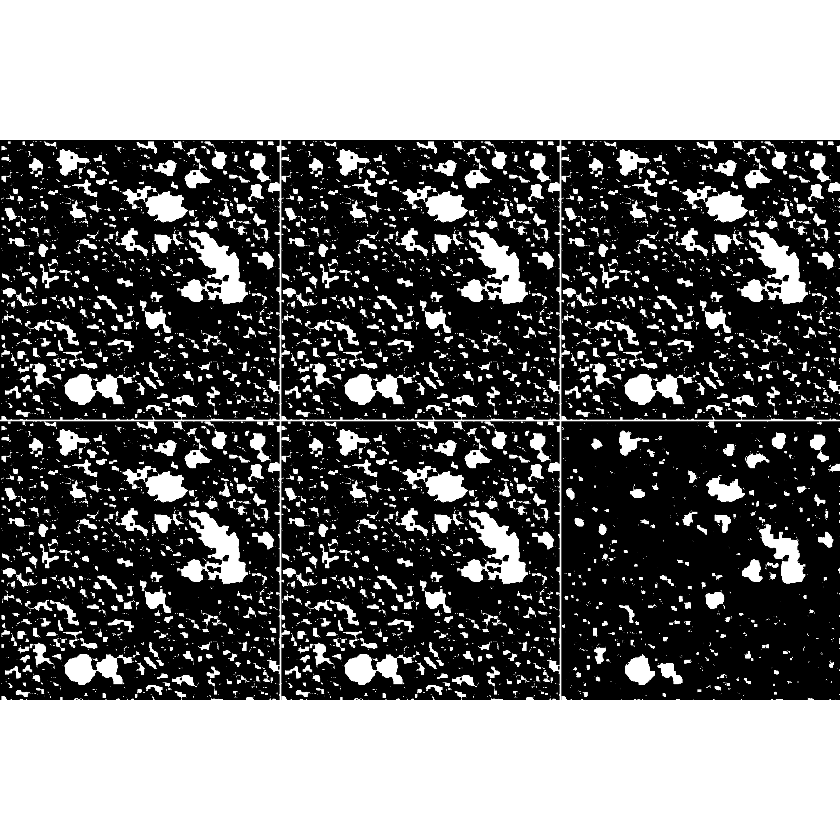
\includegraphics[width=\textwidth]{Imagenes/Resultados script morfologico/GS09.png}
     \hfill
     \caption{Resultado del filtrado con topbottom y binarizado con distintos valores de percentil, 0,1, 1, 10, 20, 50 y 90 }
    \label{topbottom}
\end{figure}

\subsubsection{Evaluación de la influencia de diferentes parámetros en los algoritmos (¿discusión?)}
Se evaluó el desempeño de los algoritmos modificando en un determinado rango el valor de distintos parámetros en cada etapa del procesamiento, para observar en qué modo se ven afectados los resultados y la vinculación que tienen los parámetros en las diferentes etapas con la resolución espacial de la imagen con la que se trabaja. En tanto en la última etapa se observó que el umbral
que se definió para separar (y por lo tanto binarizar la imagen) las copas segmentadas, en el artículo de referencia sugiere utilizar el umbral del 0,1º percentil, pero al hacer la prueba de Gridsearch con diferentes valores hasta el 90º percentil, resultaba notable que excepto el correspondiente al percentil 90º los demás resultados no eran visiblemente
diferentes.

\color{cyan} %color de texto con 70-80 % o más de avance
\subsection{RESULTADOS HOMOMÓRFICO}
Los resultados de las pruebas se exponen en la Tabla \ref{tab_homomorfico}. Allí se visualiza para distintas imágenes la cantidad de sombras detectadas, y se comparan los resultados de conteo automático con distintos tamaños de ventana, con el método de búsqueda de forma manual. Nótese el cambio de signo para el error medio entre los tamaños de ventana de 25 y de 20 píxeles, indicando que la selección de un tamaño de ventana menor resultará en una mayor 
cantidad de sombras detectadas que la que se obtiene por conteo manual. En cambio un tamaño de ventana mayor podría obviar varias sombras que serían tenidas en cuenta para el conteo manual. De acuerdo con la resolución de las imágenes de prueba, el tamaño de ventana cuadrada de 20 píxeles por lado se correspondería con un área de 100 metros cuadrados.
% Please add the following required packages to your document preamble:
% \usepackage{multirow}
\begin{table}[]
    \centering
    \begin{threeparttable}[b]
        
        \caption{Número de regiones sombreadas obtenidas por conteo manual y por el algoritmo automático de procesamiento homomórfico, como función del tamaño de ventana de exploración}
        % Please add the following required packages to your document preamble:
        \label{tab:resultados_homomorfico}
        \begin{tabular}{ccccccc}
        \hline
        \hline
                  & \textbf{Conteo}  & \multicolumn{5}{c}{\textbf{Tamaño de ventana [píxeles]}}   \\
            \textbf{Imagen}& \textbf{manual}  & \textbf{10 x 10}     & \textbf{15 x 15}     & \textbf{20 x 20 }   & \textbf{25 x 25}    & \textbf{30 x 30 }   \\ \hline
            \textbf{Par1d}  & 5  & 7      & 4      & 1     & 0     & 0     \\
            \textbf{Par2d}  & 2  & 7      & 4      & 1     & 0     & 0     \\
            \textbf{PNI1}   & 14 & 84     & 49     & 31    & 16    & 10    \\
            \textbf{PNI2}   & 14 & 48     & 35     & 20    & 14    & 7     \\
            \textbf{PNI3}   & 32 & 110    & 73     & 48    & 29    & 9     \\
            \textbf{PNI3d}  & 22 & 56     & 42     & 21    & 7     & 0     \\
            \textbf{PS1}    & 6  & 24     & 11     & 5     & 2     & 2     \\ 
            \textbf{YB1}    & 10 & 10     & 5      & 3     & 1     & 1     \\
            \textbf{YB2}    & 9  & 14     & 8      & 4     & 0     & 0     \\
            \textbf{ST1}    & 18 & 40     & 25     & 16    & 7     & 6     \\
            \textbf{ST2}    & 9  & 42     & 30     & 18    & 9     & 7     \\ \hline
            $e_{m}$\tnote{*}    & -  & -27,36 & -13,18 & -2,45 & 5,09  & 9,00  \\ 
            $\sigma^2_{e}$ \tnote{**}   & -  & 637,32  & 216,51 & 62,98 & 25,54 & 49,27 \\
           $\sigma_{e}$ \tnote{***}   & -  & 25,25  & 14,71  & 7,94  & 5,05  & 7,02  \\ \hline \hline
        \end{tabular}
        \begin{tablenotes}
        \tiny{
                \item [*]Error medio.
                \item [**]Varianza.
                \item [***] Desvío estándar.
                }
        \end{tablenotes}
  \end{threeparttable}
\end{table}
       

A los efectos de demostrar el grado de certeza del algoritmo, se comparó con la detección manual, variando el tamaño de la ventana de enmascaramiento. Se comprobó que eligiendo un tamaño de ventana de enmascaramiento igual a 20 por 20 píxeles se obtenía un acercamiento al criterio de selección manual.
En el proceso de binarización, se definió como umbral que correspondía a un valor de intensidad por encima del cual se trataba de sombras. En este caso el valor de intensidad fue de 0,75 en valores de intensidad de píxeles normalizados.
Para la selección de sombras binarizadas se recorrió la matriz de la imagen con una ventana de inspección que abarcaba 25 píxeles por lado, de modo que se evalúa un conjunto de 625 píxeles. Se estableció un umbral de 0,45 para clasificar las sombras, de modo que los recintos de píxeles blancos que superaban ese umbral eran catalogados como sombras de árboles grandes.
A los efectos de mostrar el funcionamiento del método de búsqueda y conteo de sombras, se exponen las figuras \ref{sombratorogris}, \ref{mascaraST} y \ref{seleccionadaST} en las que se visualizan la imagen satelital en escala de grises de una porción de la reserva privada Sombra de Toro, ubicada en el norte de la provincia de Misiones, la imagen binarizada luego del filtrado homomórfico y las sombras seleccionadas, respectivamente.



\begin{figure}[h!]
    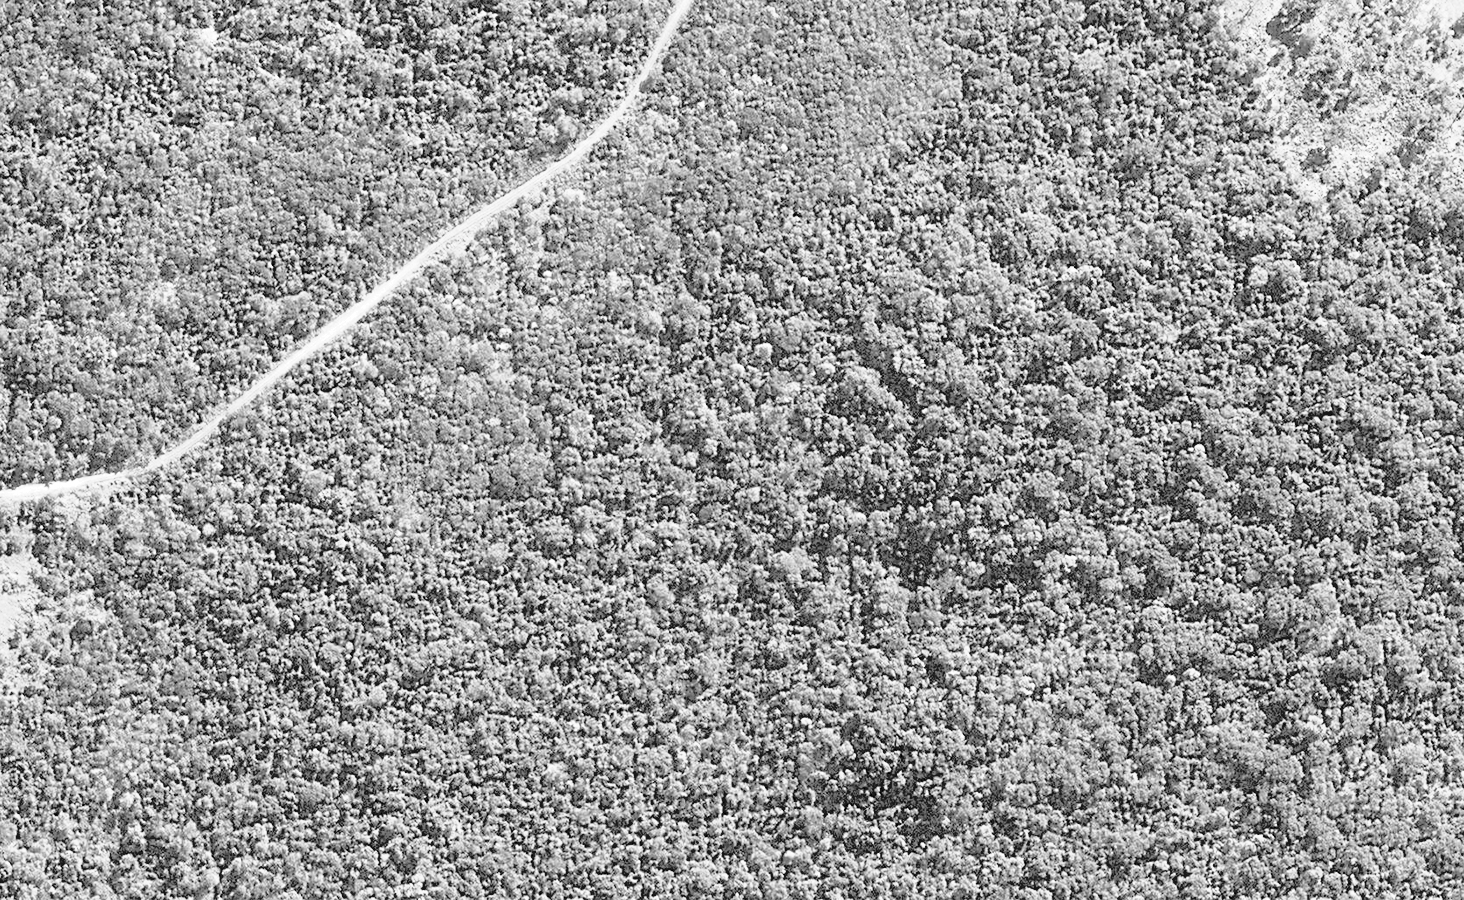
\includegraphics[width=\textwidth]{Imagenes/Homomorfico/ST2.png}
     \hfill
     \caption{Imagen aérea (satelital) de reserva privada Sombra de Toro (identificada como ST2 en la tabla), en escala de grises. Resolución de imagen de 1464 x 900 píxeles, resolución espacial de 0,5 m por pixel.}
    \label{sombratorogris}
\end{figure}

\begin{figure}[h!]
    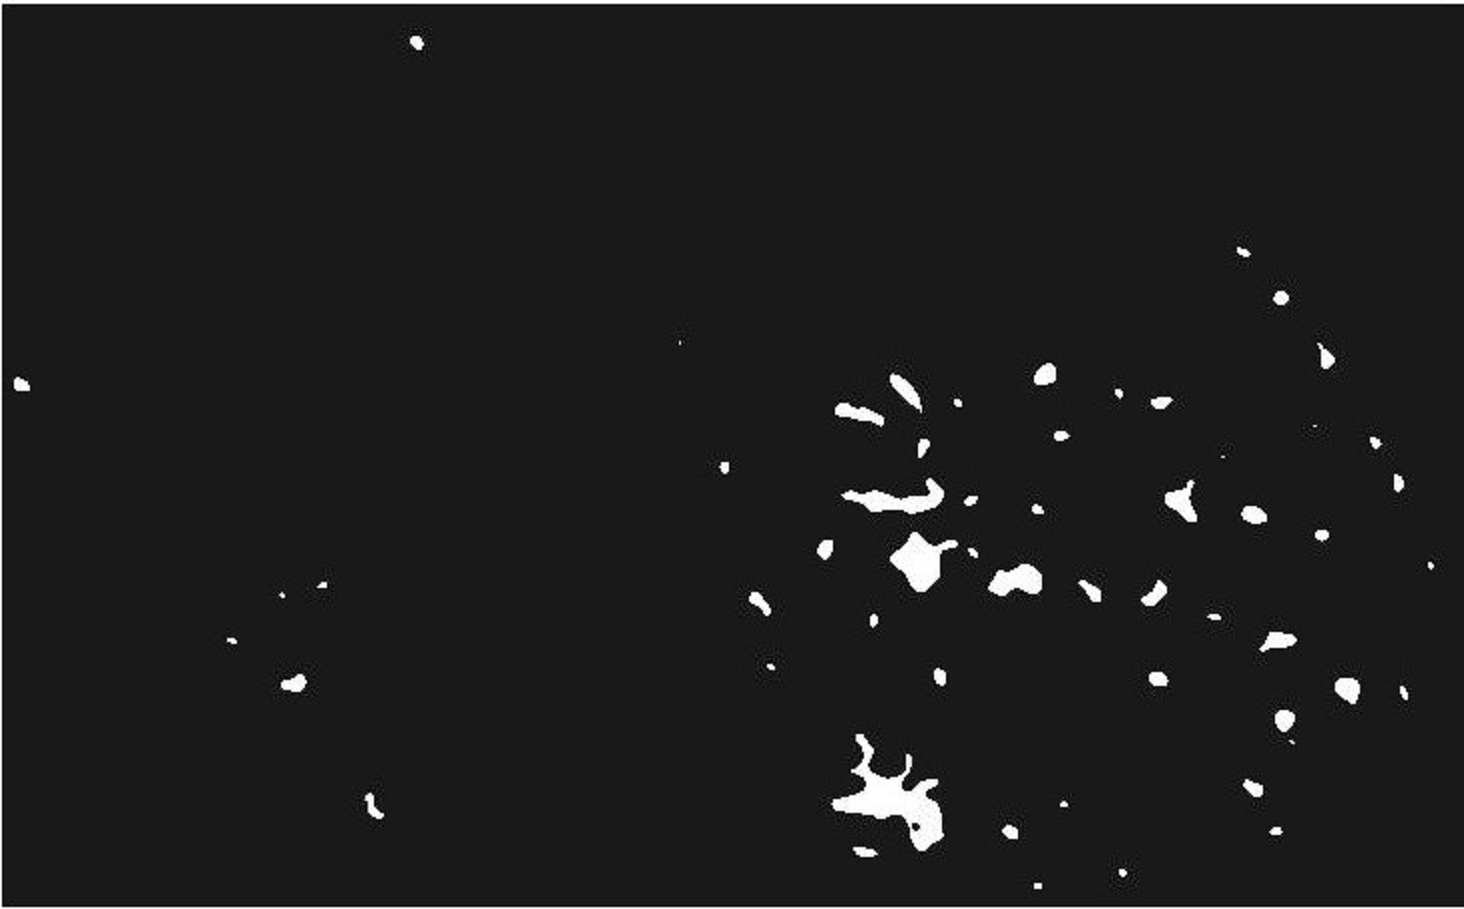
\includegraphics[width=\textwidth]{Imagenes/Homomorfico/ST2_bin.png}
     \hfill
     \caption{Máscara binaria obtenida a partir de la imagen de la figura \ref{sombratorogris} con umbral de 0,45.}
    \label{mascaraST}
\end{figure}

\begin{figure}[h!]
    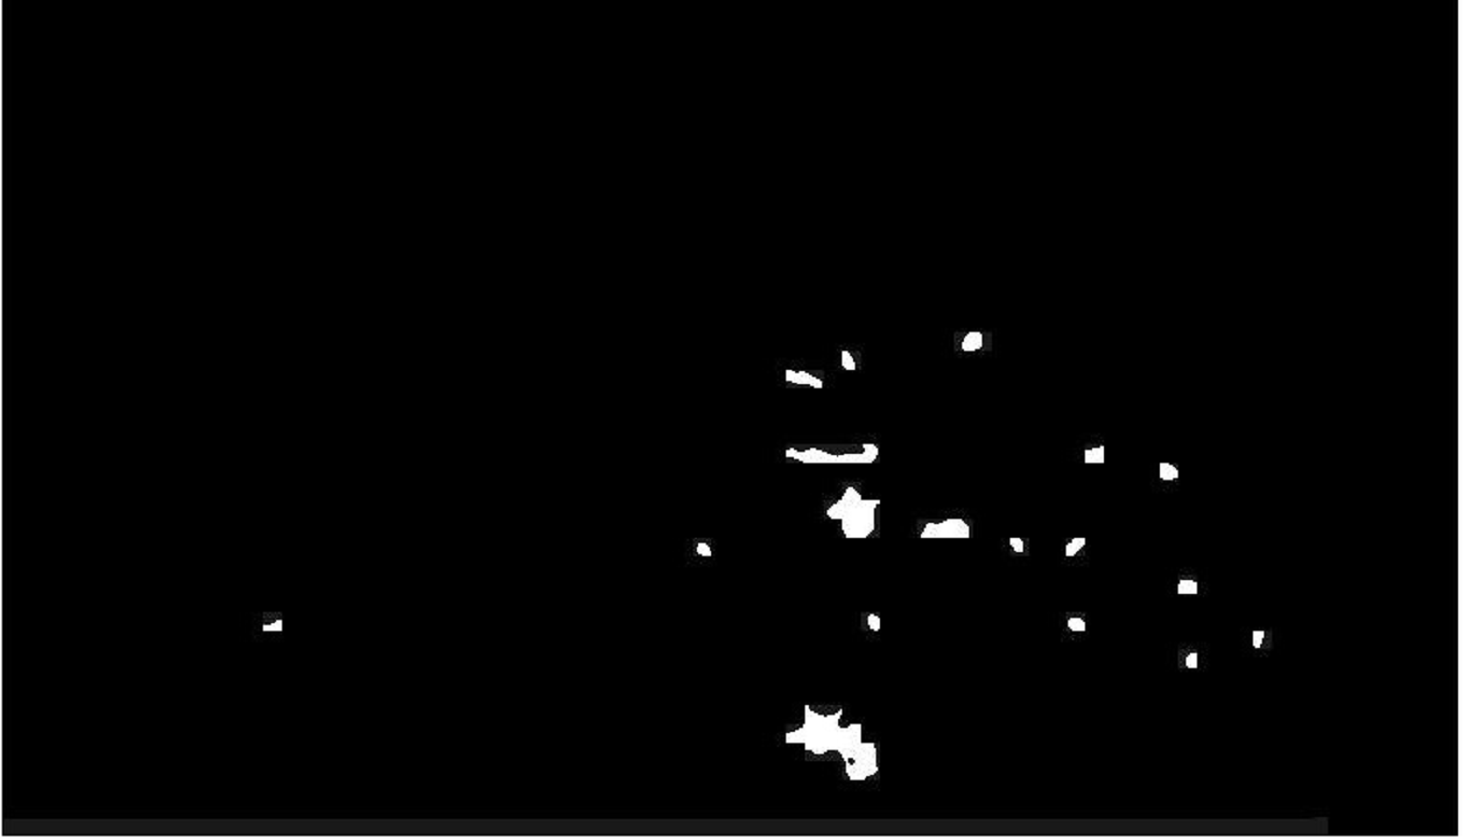
\includegraphics[width=\textwidth]{Imagenes/Homomorfico/ST2_masked.png}
     \hfill
     \caption{Sombras seleccionadas por el algoritmo a partir de la imagen de la figura \ref{mascaraST}.}
    \label{seleccionadaST}
\end{figure}
%%%%%%%%%%%%%%%%%%%%%%%%%%%%%%%%%%%%%%%%%%%%%%%%%%%%%%%%%%%%%%%%%%%%%%%%%%%%%%%%
\begin{figure}[h!]
    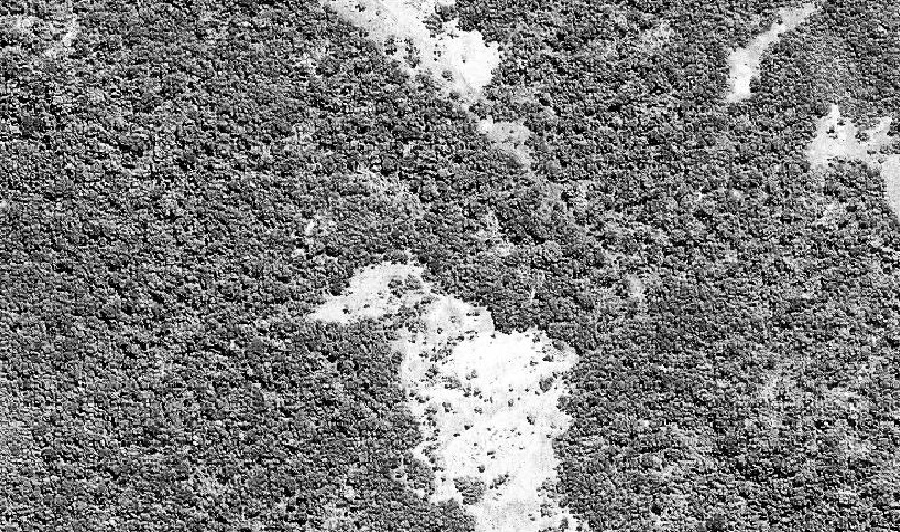
\includegraphics[width=\textwidth]{Imagenes/Homomorfico/PS1_original.jpg}
     \hfill
     \caption{Imagen aérea (satelital) de reserva Parque de la Sierra (identificada como PS1 en la tabla), en escala de grises. Resolución de imagen de 1464 x 900 píxeles, resolución espacial de 0,5 m por pixel.}
    \label{PS1}
\end{figure}

\begin{figure}[h!]
    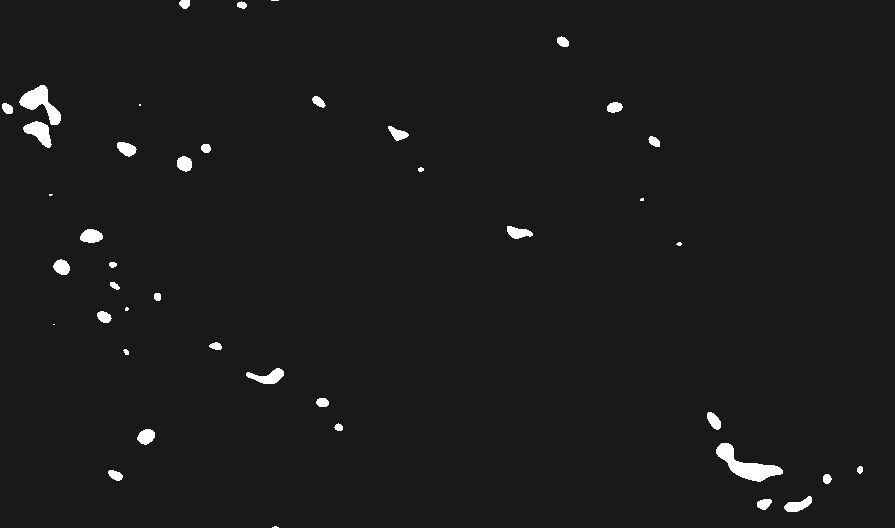
\includegraphics[width=\textwidth]{Imagenes/Homomorfico/PS1_bin.png}
     \hfill
     \caption{Máscara binaria obtenida a partir de la imagen de la figura \ref{PS1} con umbral de 0,45.}
    \label{mascaraPS1}
\end{figure}

\begin{figure}[h!]
    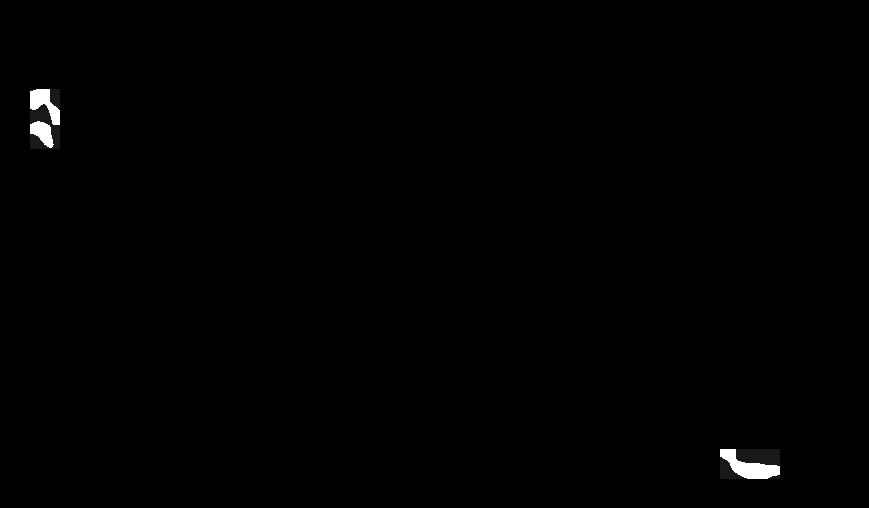
\includegraphics[width=\textwidth]{Imagenes/Homomorfico/PS1_masked.png}
     \hfill
     \caption{Sombras seleccionadas por el algoritmo a partir de la imagen de la figura \ref{mascaraPS1}.}
    \label{seleccionadaST}
\end{figure}

De acuerdo con la resolución espacial de las imágenes analizadas, el tamaño de ventana de 20 píxeles se corresponde con un área de aproximadamente cien metros cuadrados.

\color{cyan} %color de texto con 70-80 % o más de avance
\subsection{RESULTADOS IIC} \label{Resultados}
Un total de diecinueve imágenes aéreas de selva fueron consideradas para realizar el análisis. Dos de ellas representativas de los diferentes escenarios que fueron cubiertos, se muestran en las figuras \ref{calle} y \ref{tupido}. La figura \ref{calle} muestra una imagen en la que unas pocas copas de árboles se distribuyen por el área capturada, mientras que en la \ref{tupido} el dosel cubre prácticamente toda el área. La delineación manual de las sombras fue realizada como se describe en el apartado de \ref{Metodología}
Dos ejemplos de máscaras manuales se muestran en figuras \ref{contorno1} y \ref{contorno2}, con trazo rojo bordeando las regiones sombreadas. La figura \ref{superposicion} muestra el solapamiento de la máscara manual (en rojo) con la automática (en azul). En la figura \ref{p60} el valor de umbral para la máscara binaria se toma del 60º percentil de la distribución de frecuencias, mientras que en la figura \ref{p85} el valor de umbral es tomado del 85º percentil.

\begin{figure}[h!]
    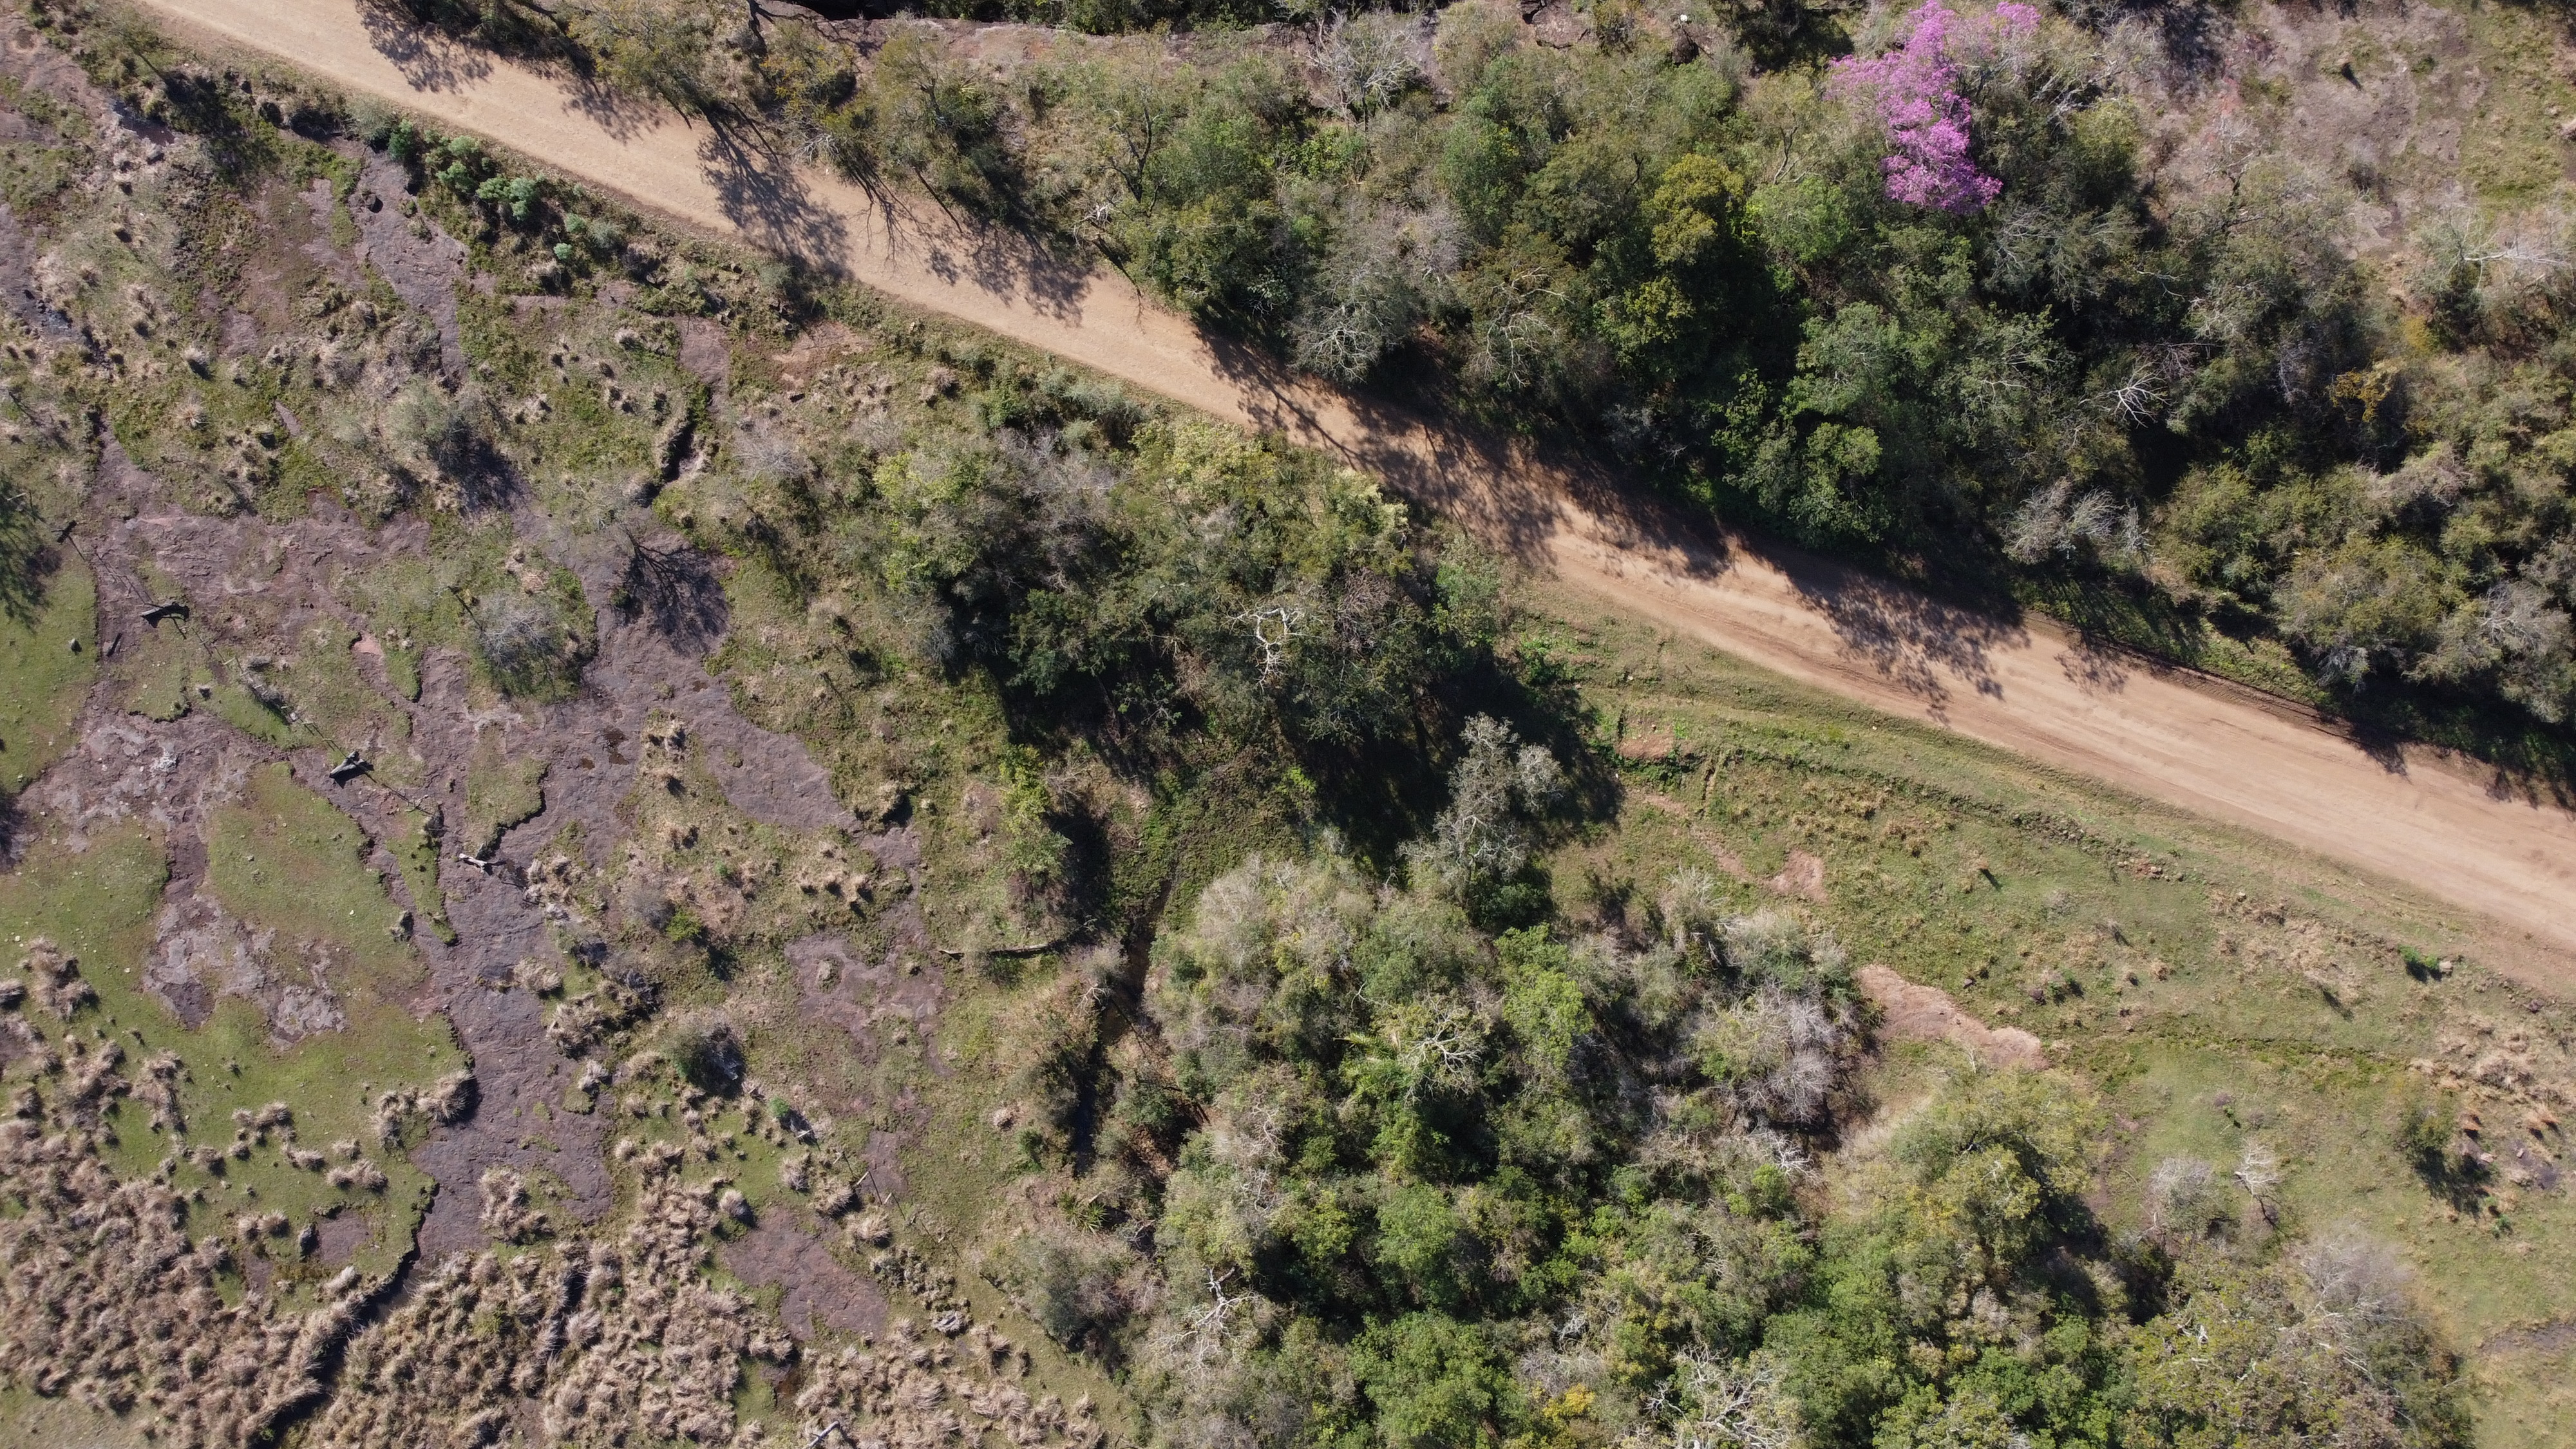
\includegraphics[width=\textwidth]{Imagenes/street.jpg}
     \hfill
     \caption{Escena capturada con pocos árboles}
    \label{calle}
\end{figure}

\begin{figure}[h!]
    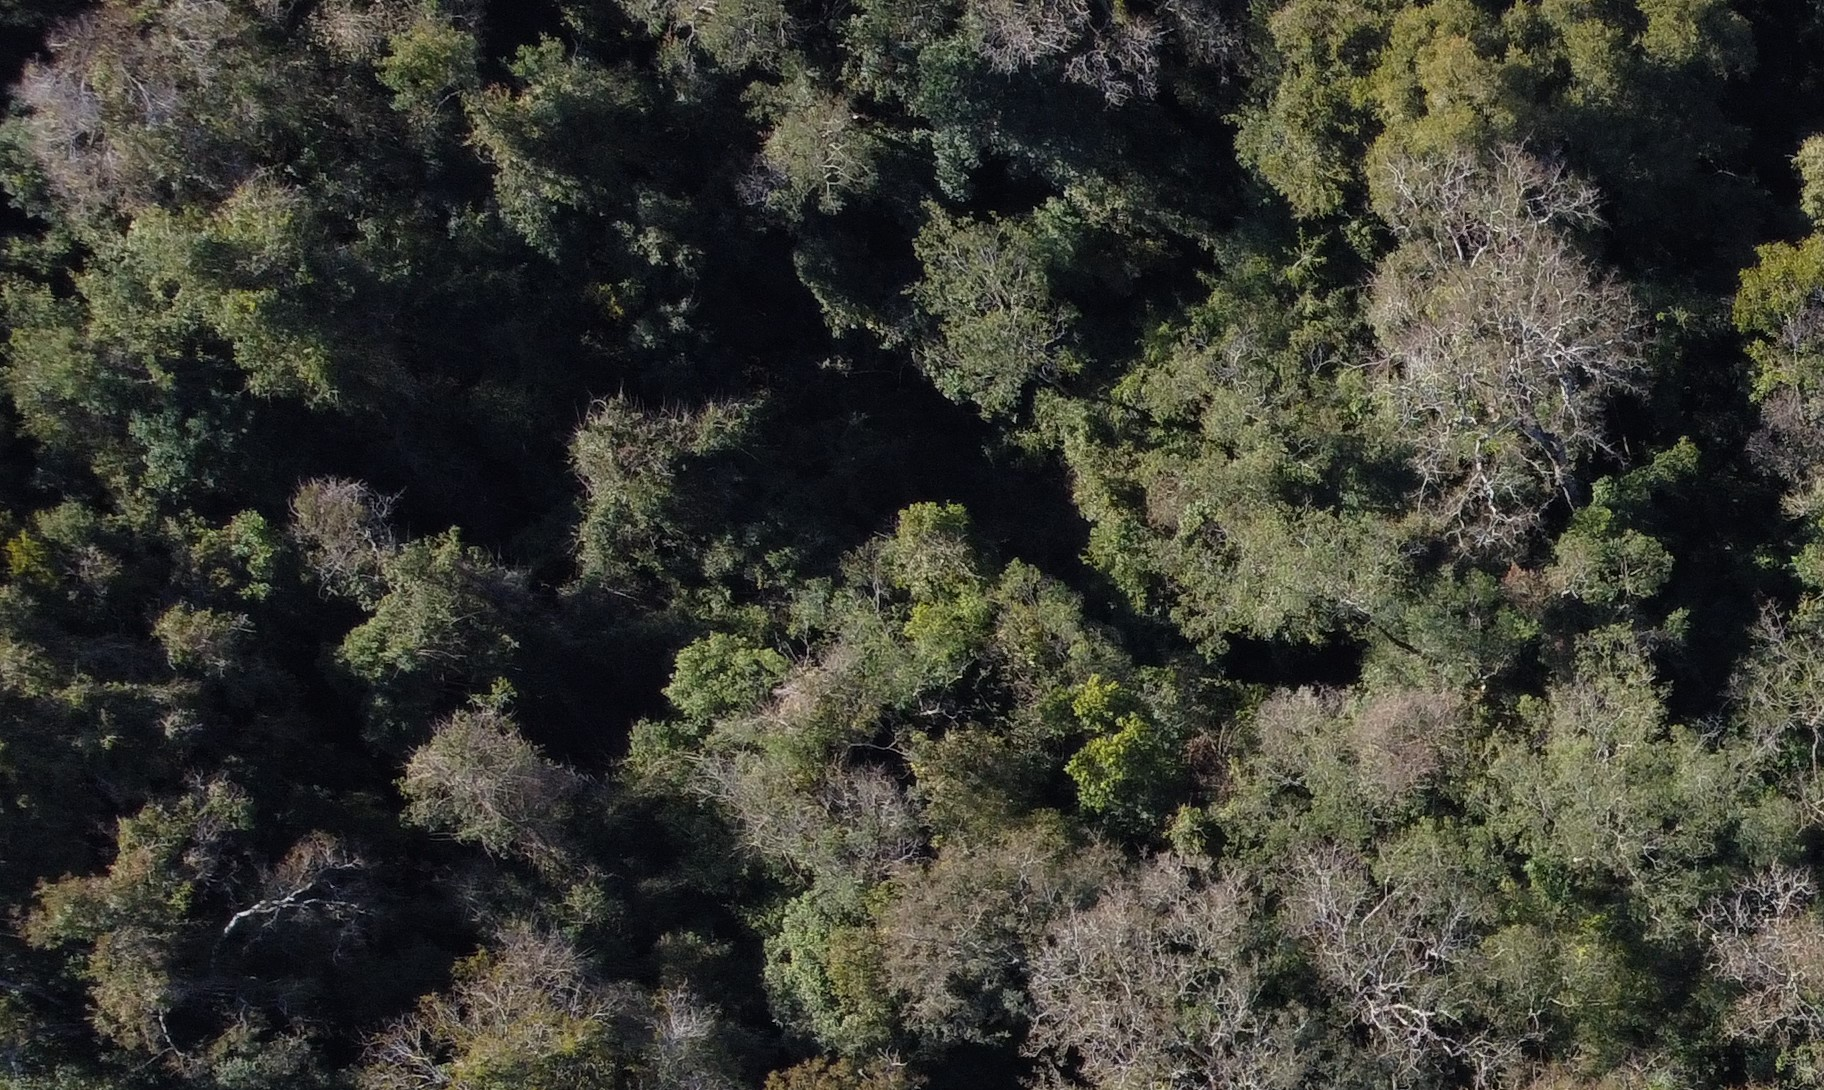
\includegraphics[width=\textwidth]{Imagenes/dense canopy.jpg}
     \hfill
     \caption{Escena capturada con dosel tupido}
    \label{tupido}
\end{figure}


\begin{figure}[h!]
    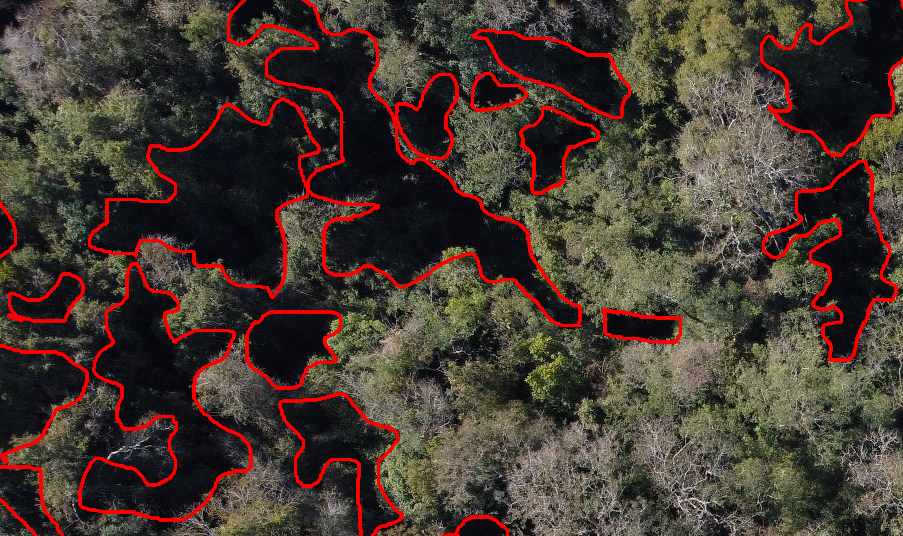
\includegraphics[width=\textwidth]{Imagenes/contours.png}
     \hfill
     \caption{Contornos de sombras en dosel tupido}
    \label{contorno1}
\end{figure}

\begin{figure}[h!]
    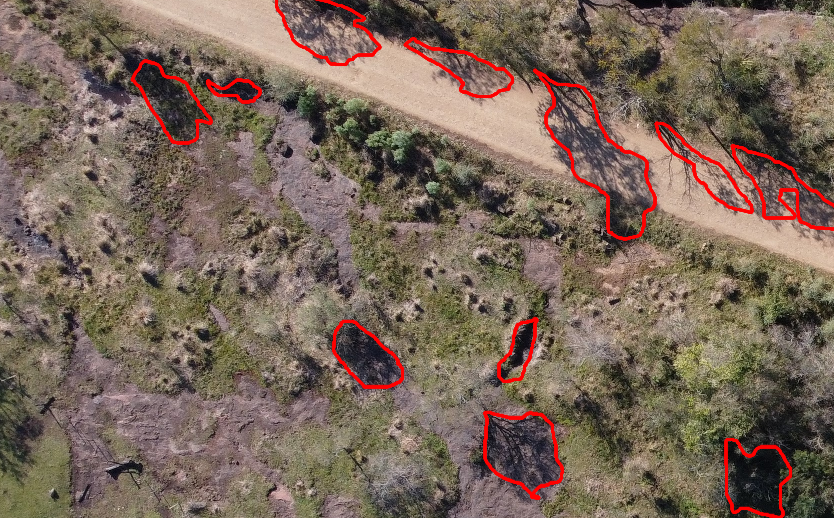
\includegraphics[width=\textwidth]{Imagenes/contours2.png}
     \hfill
     \caption{Contorno de sombras en imagen con pocos árboles}
    \label{contorno2}
\end{figure}

\begin{figure}[h!]
     \centering
     \begin{subfigure}[b]{0.5\textwidth}
         \centering
         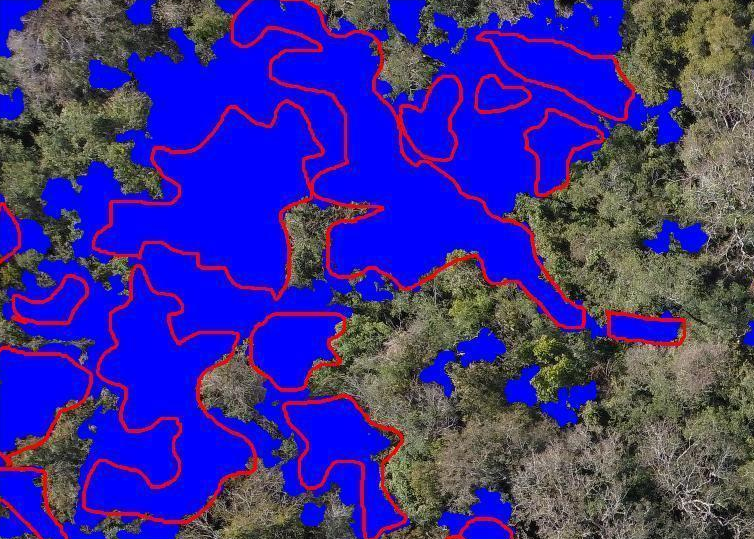
\includegraphics[width=\textwidth]{Imagenes/superposition of masks.png}
         \caption{Percentil 60º}
         \label{p60}
     \end{subfigure}
     \hfill
     
     \begin{subfigure}[b]{0.5\textwidth}
         \centering
         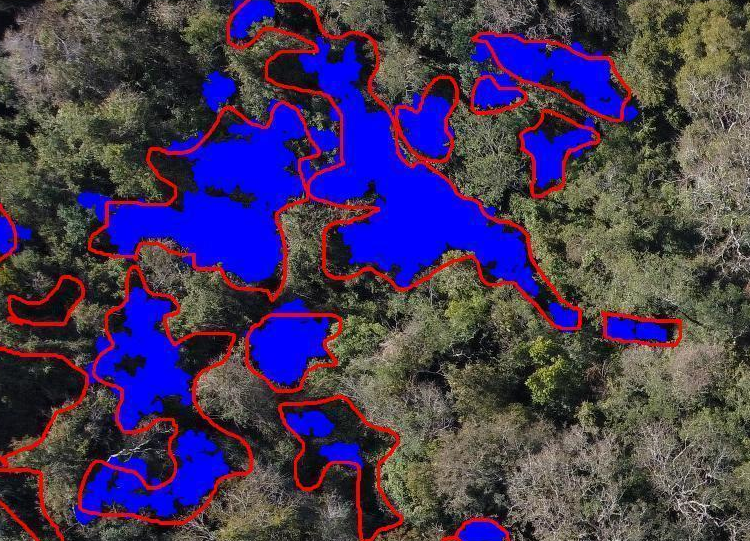
\includegraphics[width=\textwidth]{Imagenes/superposition of masks 2.png}
         \caption{Percentil 85º}
         \label{p85}
     \end{subfigure}
        \caption{Superposición de máscaras automática y manual}
        \label{superposicion}
\end{figure}

\begin{figure}[h!]
    \centering
  \begin{subfigure}[b]{0.5\textwidth}
    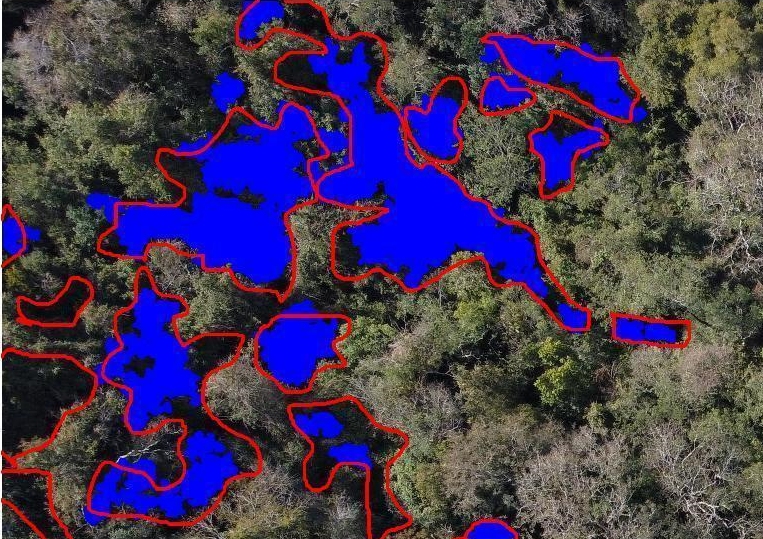
\includegraphics[width=\textwidth]{Imagenes/blue minus red 85.png}
     \hfill
     \caption{\textpsi\textsubscript{BR}}
    \label{azulrojo}
 \end{subfigure}

 \begin{subfigure}[b]{0.5\textwidth}
    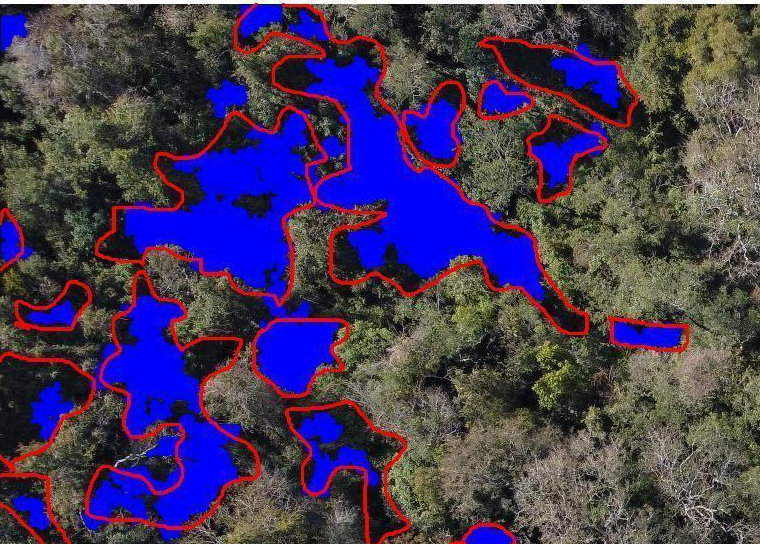
\includegraphics[width=\textwidth]{Imagenes/blue minus green 85.png}
     \hfill
     \caption{\textpsi\textsubscript{BG}}
    \label{azulverde}
 \end{subfigure}

 \begin{subfigure}[b]{0.5\textwidth}
    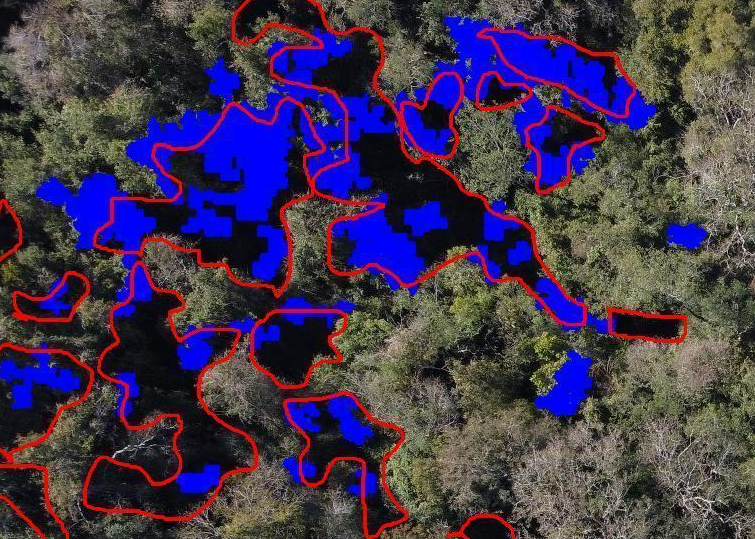
\includegraphics[width=\textwidth]{Imagenes/green minus red 85.png}
     \hfill
     \caption{\textpsi\textsubscript{GR}}
    \label{verderojo}
 \end{subfigure}
 \caption{Superposición de máscaras automática y manual}
        \label{p85BRBGGR}
\end{figure}

\begin{figure}[h!]
    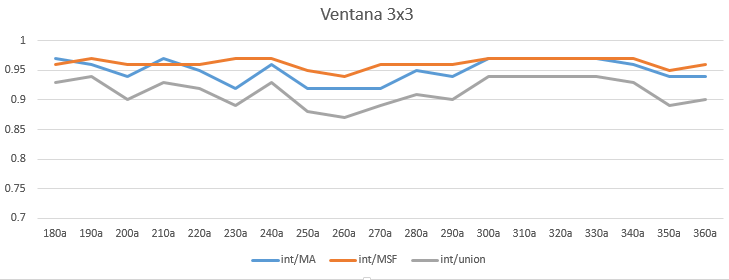
\includegraphics[width=\textwidth]{Imagenes/filter 3x3.png}
     \hfill
     \caption{Filtro 3x3}
    \label{filter3x3}
\end{figure}

\begin{figure}[h!]
    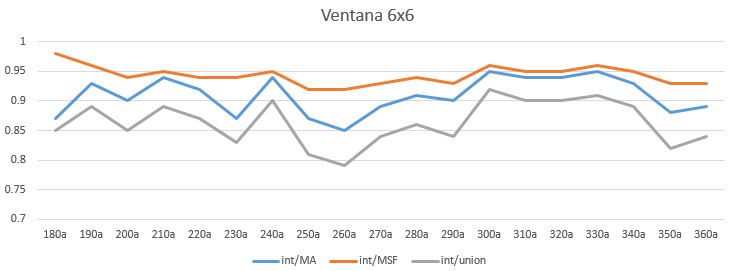
\includegraphics[width=\textwidth]{Imagenes/filter 6x6.png}
     \hfill
     \caption{6x6}
    \label{filter6x6}
\end{figure}

\begin{figure}[h!]
    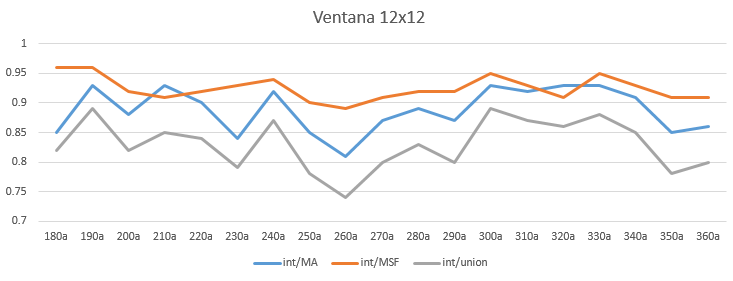
\includegraphics[width=\textwidth]{Imagenes/filter 12x12.png}
     \hfill
     \caption{12x12}
    \label{filter12x12}
\end{figure}
%%%%%%%%%%%%%%%%%%%%%%%%%%%%%%%%%%%%%%%%%%%%%%%%%%%%%%%%%%%%%%%%%%%%%%%%%


%%%%%%%%%%%%%%%%%%%%%%%%%%%%%%%%%%%%%%%%%%%%%%%%%%%%%%%%%%%%%%%%%%%%5

\begin{figure}[h!]
    \centering
  \begin{subfigure}[b]{0.8\textwidth}
    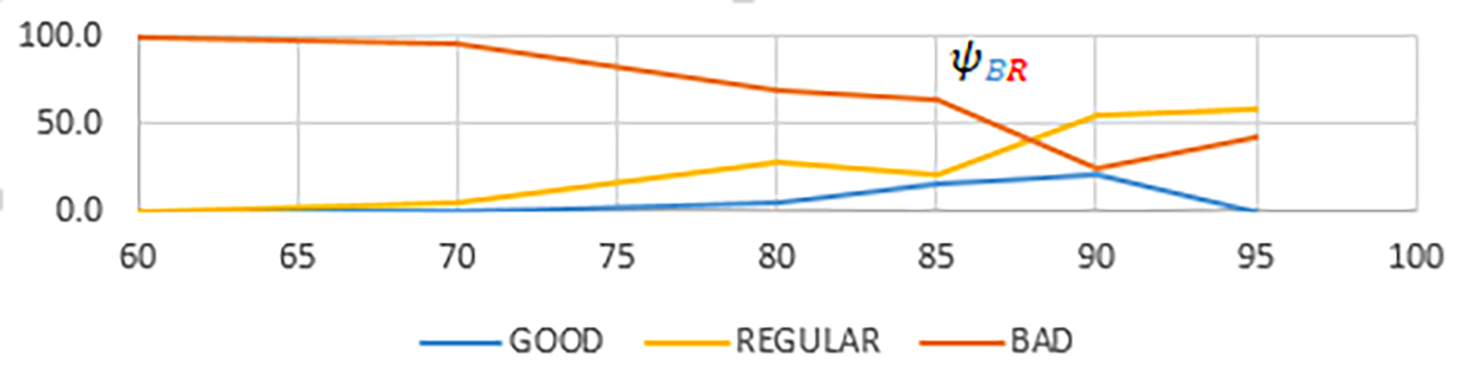
\includegraphics[width=\textwidth]{Imagenes/psiBR.png}
     \hfill
     \caption{Índice $\Psi_{BR}$}
    \label{azulrojo}
 \end{subfigure}

 \begin{subfigure}[b]{0.8\textwidth}
    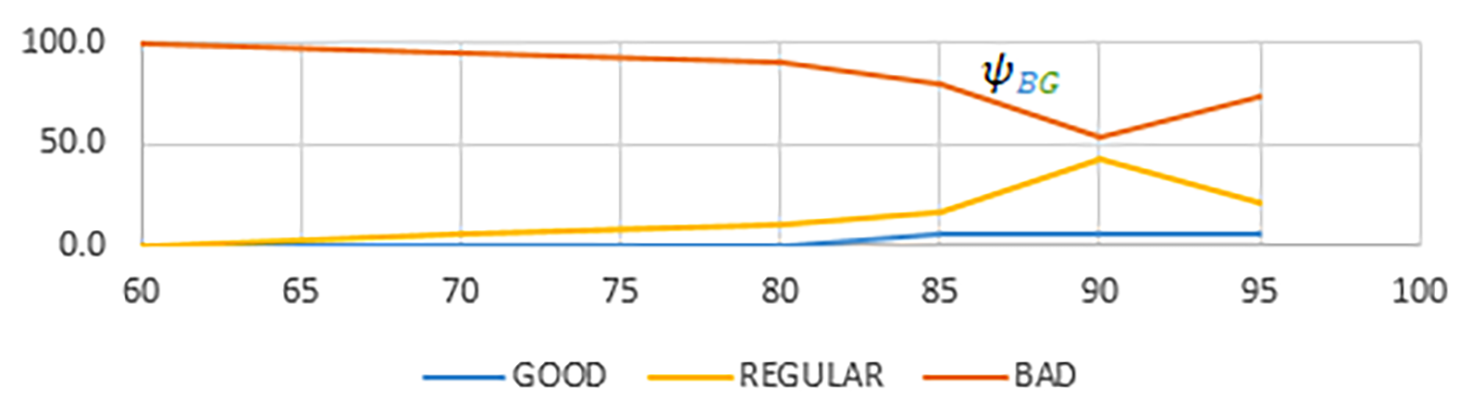
\includegraphics[width=\textwidth]{Imagenes/psiBG.png}
     \hfill
     \caption{Índice $\Psi_{BG}$}
    \label{azulverde}
 \end{subfigure}

 \begin{subfigure}[b]{0.8\textwidth}
    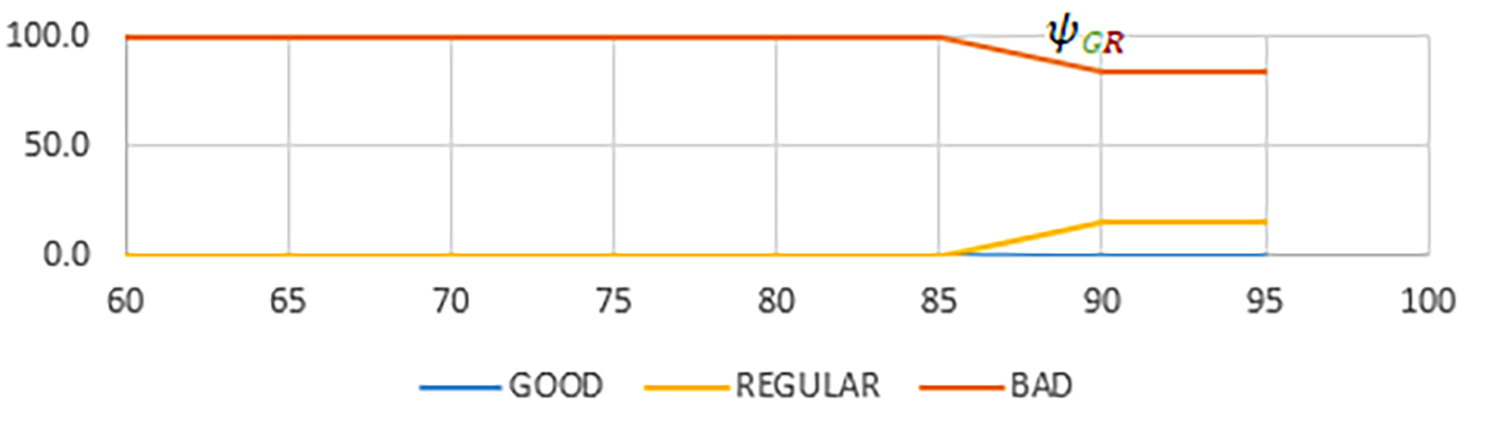
\includegraphics[width=\textwidth]{Imagenes/psiGR.png}
     \hfill
     \caption{Índice $\Psi_{GR}$}
    \label{verderojo}
 \end{subfigure}
 \caption{Comparación de máscaras automáticas con manual, para tres casos de índice invariante de color}
        \label{compara_mascara}
\end{figure}

\subsubsection{Influencia del valor de percentil y del índice invariante de color}

La figura \ref{azulrojo}, \ref{azulverde} y \ref{verderojo} muestra para la misma escena, diferentes máscaras automáticas obtenidas con diferentes configuraciones de la ecuación \ref{invariante de color}, usando tres diferentes combinaciones de canales de dos colores. La figura \ref{azulrojo} corresponde a la máscara obtenida usando la diferencia entre el canal azul menos el canal rojo $\Psi_{BR}$, la figura \ref{azulverde} usando la diferencia entre el canal azul menos el canal verde $\Psi_{BG}$ y la figura \ref{verderojo} usando la diferencia entre el canal verde menos el canal rojo $\Psi_{GR}$. En todos los casos el valor de umbral fue tomado del 85º percentil de la distribución de frecuencia. El análisis de las figuras \ref{azulrojo} a \ref{verderojo} muestra que, aplicando la ecuación \ref{invariante de color} usando ya sea la combinación de canales azul con verde $\Psi_{BG}$ o azul con rojo $\Psi_{BR}$  las máscaras automáticas resultantes para un mismo valor de percentil son de área mayor que las que corresponden al índice calculado con la diferencia entre canal verde y rojo $\Psi_{GR}$, lo que resulta en valores de QI más altos para $\Psi_{BR}$ y $\Psi_{BG}$ que para $\Psi_{GR}$. La comparación entre las distintas influencias del valor de percentil puede observarse en la figura \ref{curvas_QI}, donde resulta evidente que $QI_1$ es el más alto en el percentil bajo 60º y $QI_2$ es el más alto para el percentil alto 95º. Por otro lado el índice $QI_3$ se asemeja a una curva convexa, con valores similares a $QI_1$ para el percentil 60º y similares a $QI_2$ para el percentil 95º, cuyo valor máximo en la curva corresponde al 85º percentil. Un comportamiento similar se observa para los otros índices invariantes de color $\Psi_{BG}$ y $\Psi_{GR}$. La similitud entre QI1 y QI2 en el percentil más bajo se debe al hecho de que la máscara automática selecciona un área de sombra que resulta preponderante en la operación de unión binaria en el denominador de la ecuación \ref{qi3} en el caso de $QI_3$.
Por otro lado, el índice $QI_3$ se aproxima a $QI_1$ cuando la máscara automática selecciona un área pequeña de sombra, por lo tanto la selección manual de sombra resulta dominante en la operación de unión de máscaras en el denominador de la ecuación \ref{qi3}.
Al maximizar la intersección, se asegura la coincidencia entre las máscaras manual y automática, pero podría excederse en la máscara automática. Luego, al minimizar la unión, se puede controlar el tamaño pleno de la máscara automática. Un punto óptimo es el caso en el que el índice $QI_3$ alcanza el máximo valor. A pesar de la dispersión de los datos (ver figura \ref{curvas_QI}), se puede analizar los valores medios de los índices de calidad QI para los tres casos considerados (ver figuras \ref{psiBR}, \ref{psiBG}, \ref{psiGR}). Se observa que el valor que corresponde al 85º percentil de la distribución de frecuencia del índice invariante de color es el óptimo, ya que corresponde a un máximo del índice $QI_3$.
En el análisis de la figura \ref{quality_index}, se observan grandes similitudes, donde se grafican las relaciones entre los tres índices de calidad propuestos y un índice adicional definido como la diferencia entre el valor máximo y el mínimo entre los tres índices en función del valor de percentil usado para calcular el umbral de la máscara binaria automática. En los tres casos se detecta un valor mínimo para la curva que corresponde al índice adicional, es decir el rango (max - min), y este valor mínimo corresponde al percentil 85º. Además para los casos que usan sendas combinaciones en la ecuación \ref{invariante de color} resta de canal azul menos rojo y azul menos verde, la curva del índice $QI_3$ alcanza un valor máximo en el que corresponde al 85º percentil, mientras que este punto máximo no se hace evidente para el caso de de la combinación verde menos rojo. Por lo tanto de los cuatro índices que fueron analizados, el más conveniente es el $QI_3$, que exhibe un valor óptimo de percentil más preciso por medio del mínimo en la curva, y en los tres casos de combinaciones de canales es coincidente.

\subsubsection{Influencia del filtro de mediana en la detección automática de sombras}

La figura \ref{filter3x3}, \ref{filter6x6} y \ref{filter12x12} muestra cómo los índices que son obtenidos por las ecuaciones \ref{qi5} a \ref{qi7} son afectados por la implementación del filtro de mediana a cada imagen. En el caso del filtro de 3 x 3 píxeles, que tiene menor incidencia en los índices, los índices de calidad tienen valores mayores al 85\% para todas las imágenes. El peor desempeño lo tiene el filtro de 12 x 12, cuyo resultado comparado con la máscara automática obtenida sin filtro arrojaba una coincidencia de poco más que el 70\%.

\subsubsection{Evaluación humana de máscaras automáticas de sombra}

En este trabajo los resultados del algoritmo se comparan con la selección manual llevada a cabo por expertos. Partiendo de que no hay una base de certeza absoluta (los expertos son personas humanas y por lo tanto proclives a errores de omisión o comisión), existe una limitación en el índice de calidad que se basa en este aspecto. El criterio para la selección manual de parte de los expertos depende de su particular percepción de la imagen, variando según el contexto. Por otro lado el algoritmo se basa en el cálculo de un índice y la definición de un valor umbral, obtenido de una serie de experimentos con imágenes de un determinado tipo. En otros contextos con otro tipo de imágenes el valor de umbral no sería el mismo, incluso la combinación de bandas usadas en la ecuación \ref{invariante de color} para obtener el índice sería diferente.
Luego de generar un conjunto de máscaras correspondientes a cada uno de los seis percentiles usando los tres índices invariantes de color de las ecuaciones \ref{psibr} a \ref{psigr} para las 19 imágenes seleccionadas, las 342 máscaras resultantes fueron comparadas con las obtenidas manualmente. Superponiendo ambas, la máscara automática y la manual sobre la imagen original, se evaluó la calidad de las similitudes mutuas, asignando un calificativo en tres niveles, "bueno", "regular" y "malo". Los resultados se muestran en la tabla \ref{tablaiic} y en la figura \ref{}. Tal como se puede apreciar, para los tres índices invariantes de color se puede observar un mínimo en el nivel "malo" alrededor del percentil 90º. Para los niveles "regular" y "bueno", sin embargo, el mínimo no es tan claro, lo cual puede ser atribuido a cierta subjetividad de los observadores expertos.

%%%%%%%%%%%%%%%%%%%%%%%%%%%%%%%%%%%%%%%%% TABLA %%%%%%%%%%%%%%%%%%%%%%%%%%%%%%%%%%%%%%%%%%%%%%%%%%%%%%%%%
\begin{table}[H]
    \centering
    \caption{Evaluación de la superposición de ambas máscaras, manual y automática,}
    \begin{tabular}{|c|c|c|c|c|c|c|c|}
       \hline
        ÍNDICE INVARIANTE DE COLOR & \multicolumn{6}{ |c|}{\textpsi \textsubscript{BR}}\\%\multicolumn{6}{ }{ |c|} \\
        \hline
        PERCENTIL & 60 & 70 & 80 & 85 & 90 & 95\\
        \hline
        BUENO & 0,0 & 0,0 & 4,5 & 15,8 & 20,5 & 0,0\\
        \hline
        REGULAR & 0,0 & 4,5 & 27,3 & 21,1 & 54,5 & 57,9\\
        \hline
        MALO & 100,0 & 95,5 & 68,2 & 63,2 & 25,0 & 42,1\\
        \hline
        ÍNDICE INVARIANTE DE COLOR & \multicolumn{6}{ |c|}{\textpsi \textsubscript{BG}}\\
        \hline
        PERCENTIL & 60 & 70 & 80 & 85 & 90 & 95\\
        \hline
        BUENO & 0,0 & 0,0 & 0,0 & 5,3 & 5,3 & 5,3\\
        \hline
        REGULAR & 0,0 & 5,3 & 10,5 & 15,8 & 42,1 & 21,1\\
        \hline
        MALO & 100,0 & 94,7 & 89,5 & 78,9 & 52,6 & 73,7\\
        \hline
        ÍNDICE INVARIANTE DE COLOR & \multicolumn{6}{|c|}{ \textpsi \textsubscript{GR}}\\
        \hline
        PERCENTIL & 60 & 70 & 80 & 85 & 90 & 95\\
        \hline
        BUENO & 0,0 & 0,0 & 0,0 & 0,0 & 0,0 & 0,0\\
        \hline
        REGULAR & 0,0 & 0,0 & 0,0 & 0,0 & 15,8 & 15,8\\
        \hline
        MALO & 100,0 & 100,0 & 100,0 & 100,0 & 84,2 & 84,2\\
        \hline
    \end{tabular}
    \\
    \raggedleft
    \label{tablaiic}
\end{table}
%%%%%%%%%%%%%%%%%%%%%%%%%%%%%%%%%%%%%%%%%%%%%%%%%%%%%%%%%%%%%%%%%%%%%%%%%%%%%%%%%%%%%%%%%%%%%%%%%%%%%%%%% 

%%%%%%%%%%%%%%%%%%%%%%%%%%%%%%%%%%%%%%%%%%%%%%
\begin{figure}[h!]
     \centering
     \begin{subfigure}[b]{\textwidth}
         \centering
         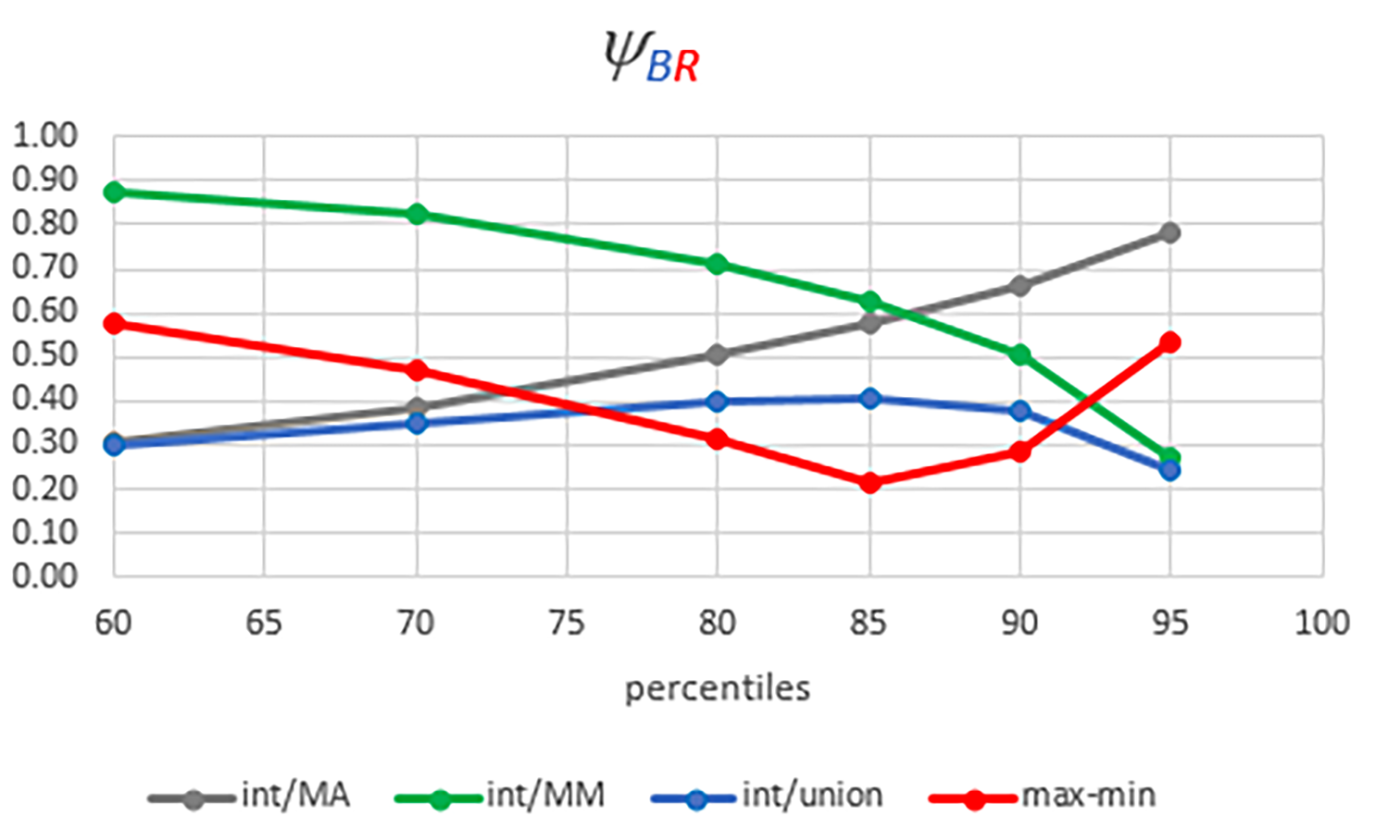
\includegraphics[width=\textwidth]{Imagenes/qibr.png}
         \caption{\textpsi \textsubscript{BR}}
         \label{psiBR}
     \end{subfigure}
     \hfill
     \begin{subfigure}[b]{\textwidth}
         \centering
         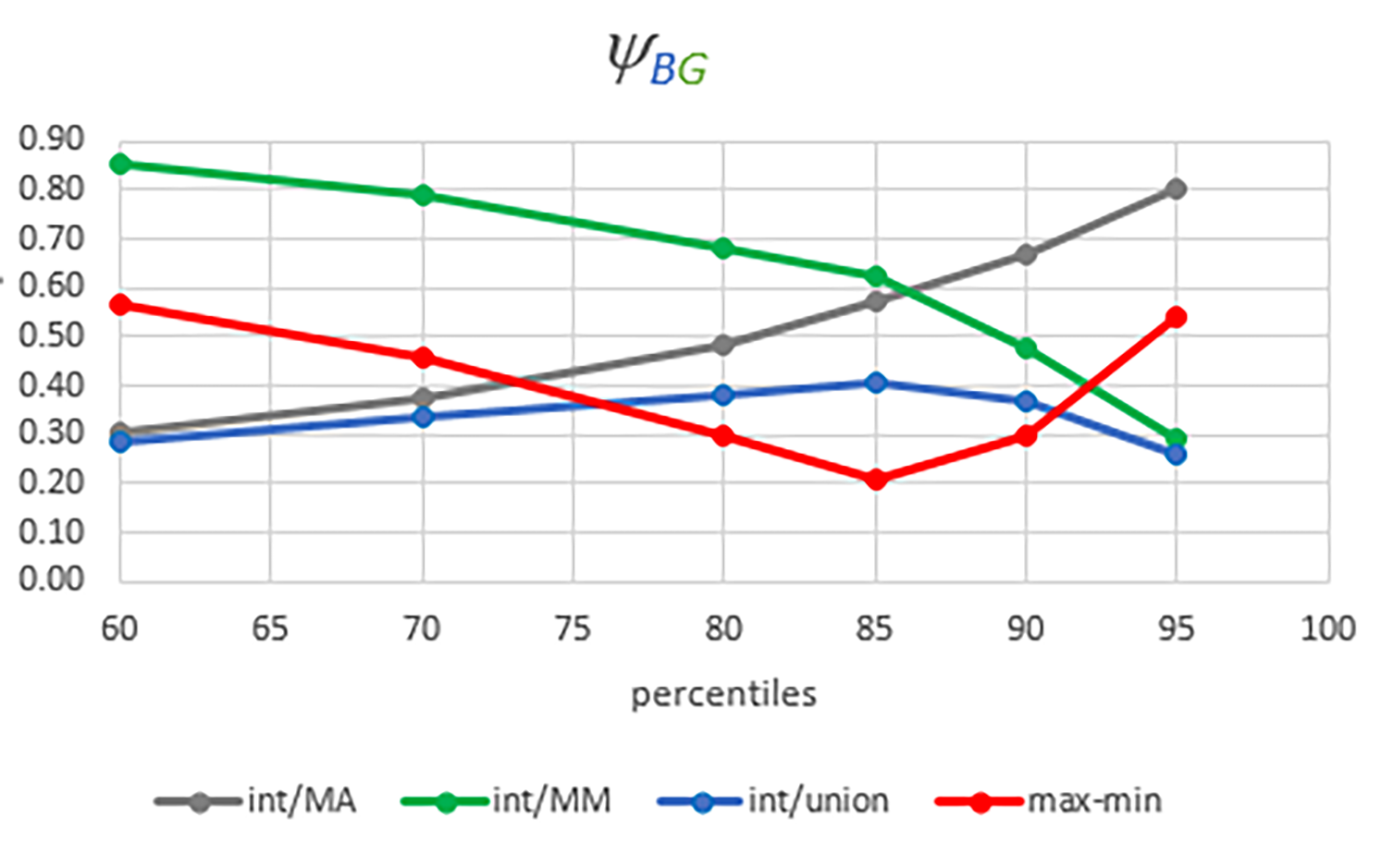
\includegraphics[width=\textwidth]{Imagenes/qibg.png}
         \caption{\textpsi \textsubscript{BG}}
         \label{psiBG}
     \end{subfigure}
     \hfill
     \begin{subfigure}[b]{\textwidth}
         \centering
         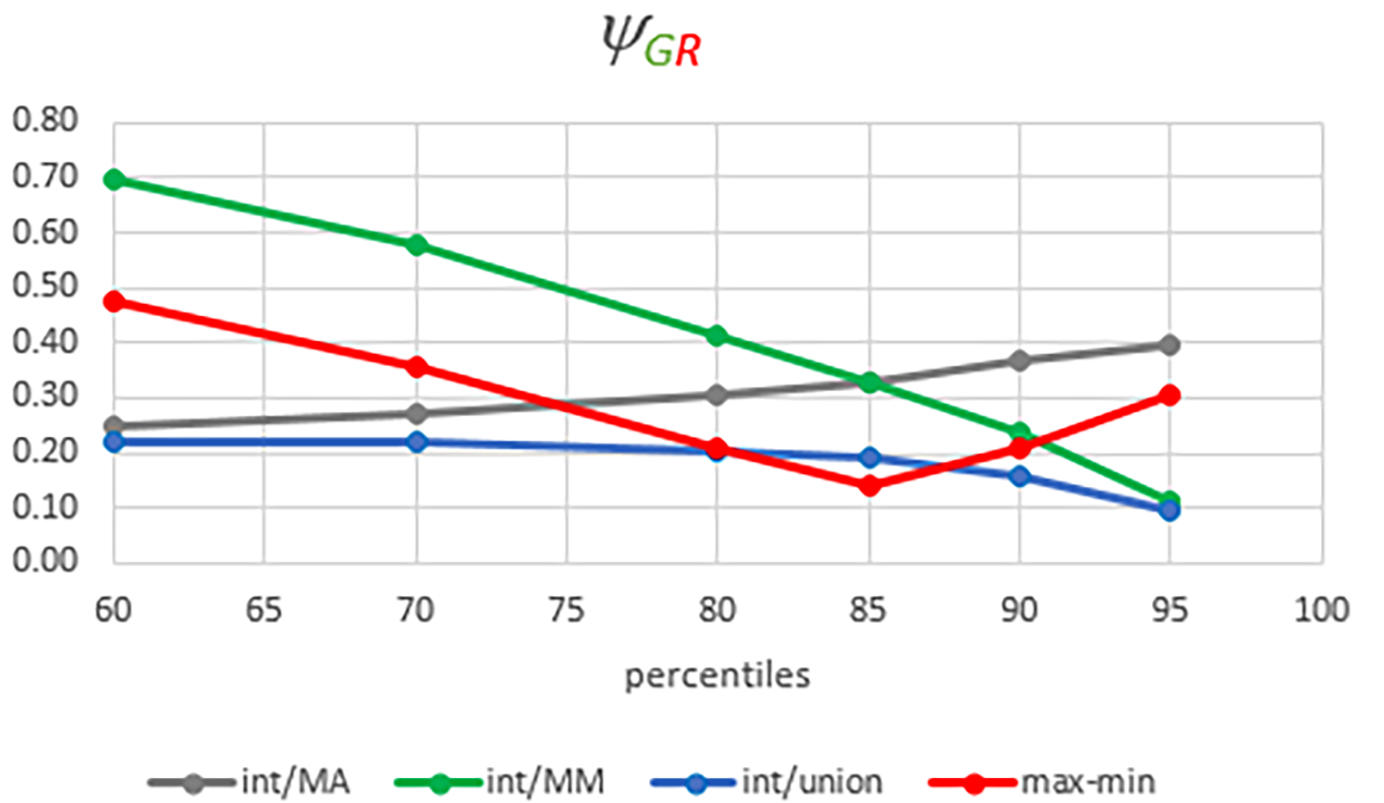
\includegraphics[width=\textwidth]{Imagenes/qigr.png}
         \caption{\textpsi \textsubscript{GR}}
         \label{psiGR}
     \end{subfigure}
        \caption{Índice de calidad}
        \label{quality_index}
\end{figure}

%tamaño
\begin{figure} [h!]
         \centering
         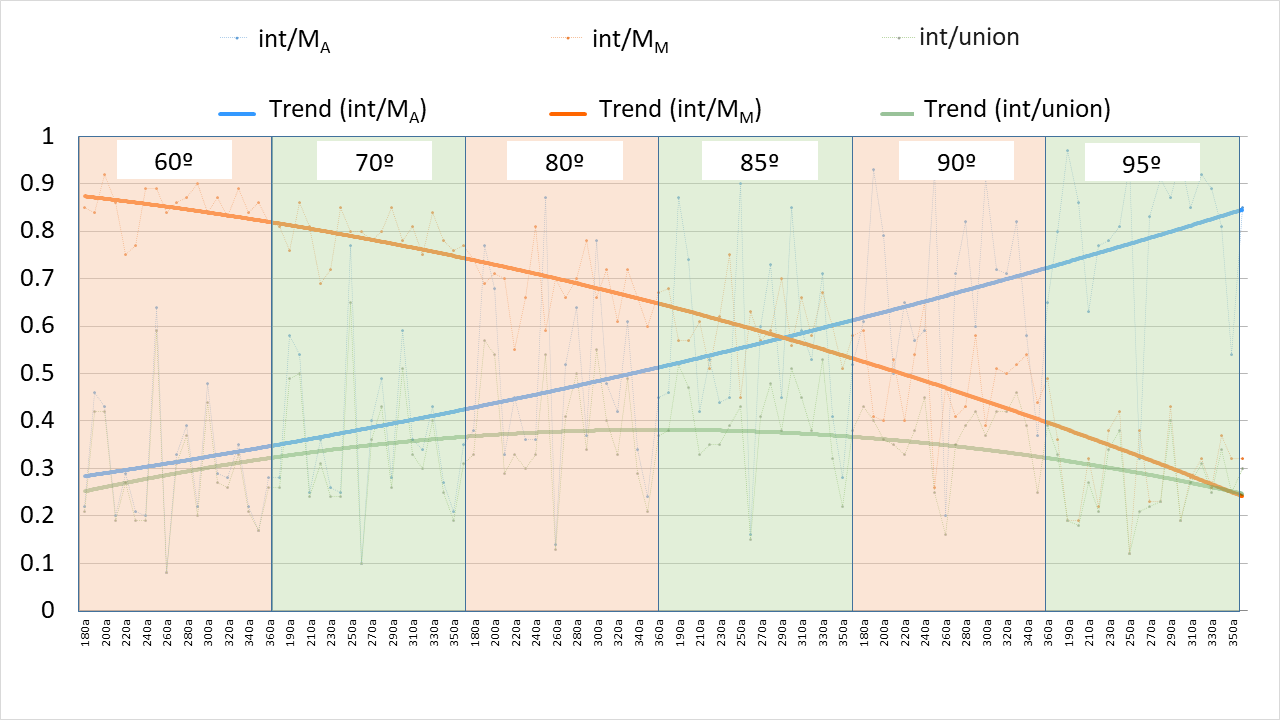
\includegraphics[width=\textwidth]{Imagenes/grafico.png}
         \hfill
         \caption{Curvas índice de calidad}
        \label{curvas_QI}
\end{figure}

%%%%%%%%%%%%%%%%%%%%%%%%%%%%%%%%%%%%%%%%%%%%%%
\begin{figure}[h!]
     \centering
     \begin{subfigure}[b]{\textwidth}
         \centering
         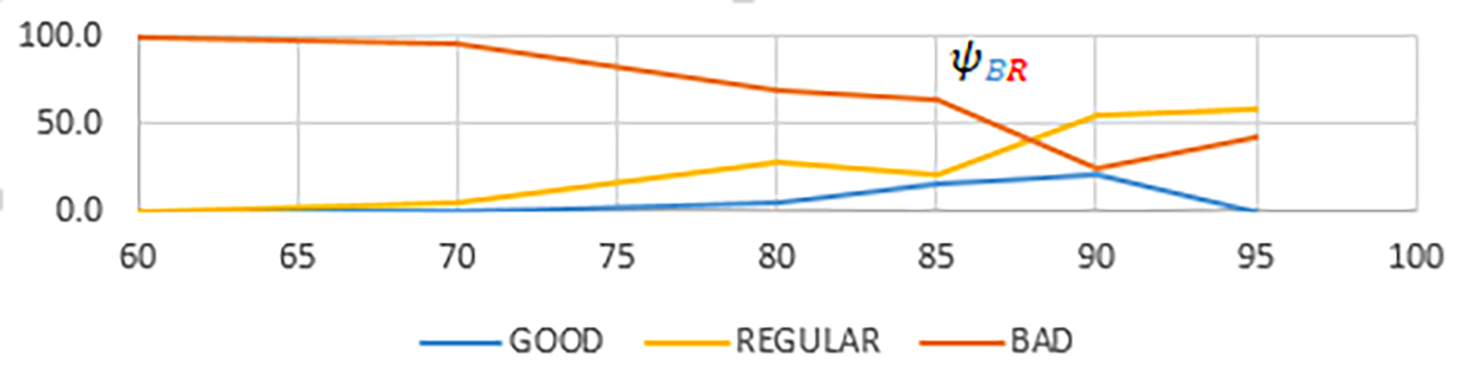
\includegraphics[width=\textwidth]{Imagenes/psiBR.png}
         \caption{\textpsi \textsubscript{BR}}
         \label{psiBR}
     \end{subfigure}
     \hfill
     \begin{subfigure}[b]{\textwidth}
         \centering
         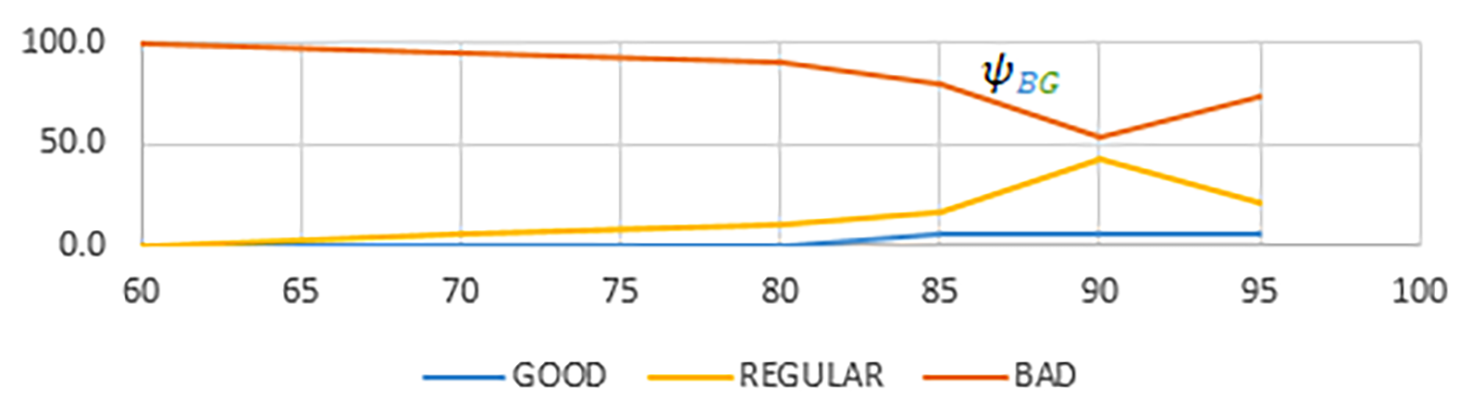
\includegraphics[width=\textwidth]{Imagenes/psiBG.png}
         \caption{\textpsi \textsubscript{BG}}
         \label{psiBG}
     \end{subfigure}
     \hfill
     \begin{subfigure}[b]{\textwidth}
         \centering
         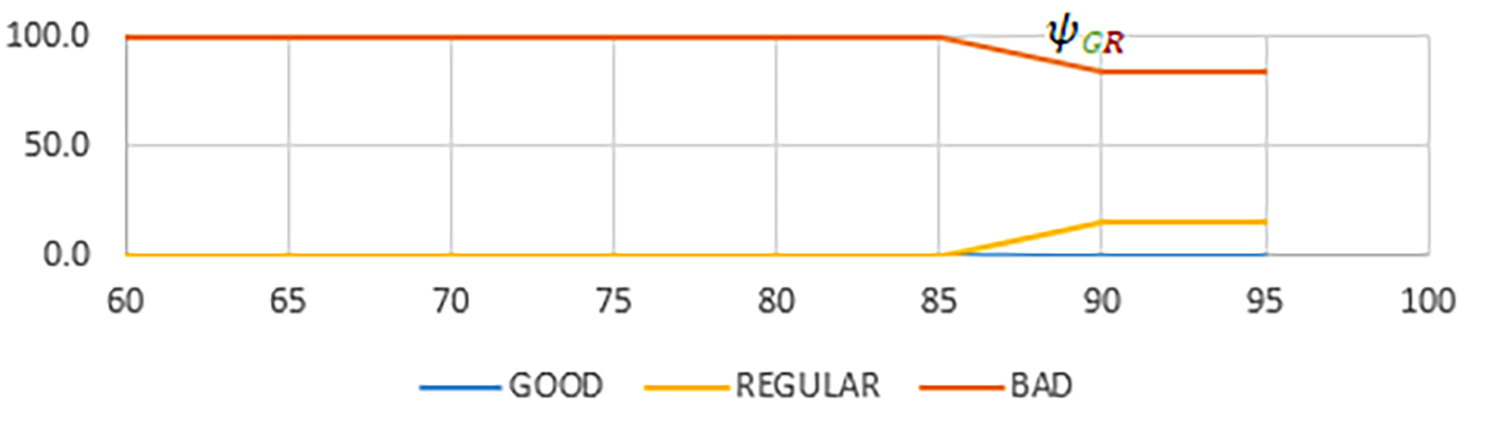
\includegraphics[width=\textwidth]{Imagenes/psiGR.png}
         \caption{\textpsi \textsubscript{GR}}
         \label{psiGR}
     \end{subfigure}
        \caption{Qualification of overlapping of both, manual and automatic masks by human experts}
        \label{humanscoring}
\end{figure} 


\subsubsection{Validación IIC} \label{Validacion}
Superponiendo a una imagen las dos máscaras, una obtenida en forma manual y otra en forma automática, tres expertos realizaron un análisis, calificando el grado de ajuste entre ambas máscaras como "bueno", "regular" o "malo". Este procedimiento fue aplicado a cada una de las 19 imágenes analizadas, de modo que se obtuvieron 19 máscaras automáticas por medio del algoritmo para ser comparadas con las respectivas máscaras obtenidas en forma manual. Las superposiciones calificadas como "buenas" o "regulares" son usadas para seleccionar la mejor máscara automática. Un procedimiento similar se siguió para evaluar el filtrado de la imagen.

%%%%%%%%%%%%%%%%%%%%%%%%%%%%%%%%%%%%%%%%%%%%%%%%%%%%%%%%%%%%%%%%%%%%%%%%%%%%%%%%%%%%%%%%%%%%%%%%%%%%%%%%%%%%%%%%%%%%%%%%%%%%%%
\color{orange} %ver si esto lo dejamos o no...
\subsection{C3-Filtros de texturas (probados con fantomas)}
Mediante el filtrado por textura puede implementarse una segmentación o clasificación en imágenes. Se hicieron varias pruebas con imágenes simuladas (cuadrados y rombos)
\subsection{C4-Mapas autoorganizados (clasificación no supervisada)}
\subsection{C5-IIC: Análisis de efecto de bandas utilizadas (sombras)}
Informe 1
Se realizaron pruebas del algoritmo sobre distintas imágenes que contienen sombra para ver su desempeño en la selección automática de sombras. Para todos los casos se aplicó para definir el umbral de binarización el correspondiente al percentil 85 de la distribución de frecuencias del índice invariante de color calculado por la ecuación \ref{invariante de color 1}:
 %%%%%%%%%%%%%%%%%%%%%%%%%%%%%%%%%%%%%% ECUACIÓN %%%%%%%%%%%%%%%%%%%%%%%%%%%%%%%%%%%%%%%%%%%%%%%%%%%%%%%%%
\\
\begin{equation}
	\psi=\frac{4}{\pi} arctan\left(\frac{B\textsubscript{1}-B\textsubscript{2}}{B\textsubscript{1}+B\textsubscript{2}}\right),\label{invariante de color 1}
\end{equation}
\\
%%%%%%%%%%%%%%%%%%%%%%%%%%%%%%%%%%%%%%%%%%%%%%%%%%%%%%%%%%%%%%%%%%%%%%%%%%%%%%%%%%%%%%%%%%%%%%%%%%%%%%%%%
La imagen de la izquierda se procesó con la combinación de las bandas azul y verde, la de la derecha con la combinación azul y rojo.
Se observa que hay mucha similitud en las áreas marcadas, no obstante los diferentes valores de binarización, obtenidos por criterio del 85to percentil de la distribución de frecuencias de los valores de índice invariante de color hallados para cada combinación de bandas.
\\
\\
Informe 2
Aplicando el algoritmo sobre una imagen seleccionada que contiene sombras, usando la ecuación \ref{invariante de color 2} en la combinación de bandas verde y roja y sin utilizar el criterio de percentil para definir el umbral de binarización:
%%%%%%%%%%%%%%%%%%%%%%%%%%%%%%%%%%%%%% ECUACIÓN %%%%%%%%%%%%%%%%%%%%%%%%%%%%%%%%%%%%%%%%%%%%%%%%%%%%%%%%%
\\
\begin{equation}
	\psi=\frac{4}{\pi} arctan\left(\frac{B\textsubscript{1}-B\textsubscript{2}}{B\textsubscript{1}+B\textsubscript{2}}\right),\label{invariante de color2}
\end{equation}
\\
%%%%%%%%%%%%%%%%%%%%%%%%%%%%%%%%%%%%%%%%%%%%%%%%%%%%%%%%%%%%%%%%%%%%%%%%%%%%%%%%%%%%%%%%%%%%%%%%%%%%%%%%%
Observando la imagen con la máscara superpuesta en color azul se nota una marcación altamente coincidente con la que corresponde al área sombreada. Además, mediante el gráfico de histograma de frecuencias del índice invariante de color es posible advertir el valle entre dos picos situado en torno al valor 0,2 el cual fue usado como umbral de binarización.
\\
\\
Informe 3

Tal como surge de la ecuación 1, las posibilidades de combinar dos entre tres bandas de color resultan en seis diferentes índices invariantes de color para una imagen dada. Lo que resulta notorio es que a priori no se sabe cuál de esas seis resulta la más adecuada para constituir la máscara de selección automática de sombras. 
\color{black}
